\documentclass[a4paper,12pt,oneside]{book}

\input{config/packages.tex}
\input{config/settings.tex}
\input{config/abbreviations.tex}
\usepackage{setspace}
\usepackage{multirow}

\usepackage{graphicx} 
\usepackage{caption,subcaption}


% Remove these two lines for page break after sections
% \usepackage{titlesec}
% \titleclass{\chapter}{straight}

\begin{document}
\onehalfspacing

\frontmatter
\pagestyle{plain}
% Uppercase Roman page numbering for front matter
\pagenumbering{Roman}

\begin{titlepage}
  \thispagestyle{empty}

  \makebox[\textwidth]{
    % Logo on the left:
    % \includegraphics[height=1.5cm]{figures/logos/hm-logo.png}
    \hfill
    % Logo on the right:
    \includegraphics[height=1.6cm]{figures/logos/hm-logo.png}
  }

  \vspace{2cm}

  \begin{center}
    {\LARGE \textbf{Erkennung KI-generierter Texte auf Reddit} \\}
    \vspace{0.5cm}
    {\large Eine experimentelle Evaluation von Machine-Learning-Detektoren}

    \vspace{1.2cm}
    {\large \textbf{Bachelorarbeit} \\}
    \vspace{0.2cm}
    zur Erlangung des akademischen Grades Bachelor of Science (B.Sc.)

    \vspace{1.2cm}
    Vorgelegt an der \\
    Hochschule München \\
    Fakultät für Informatik und Mathematik

    \vspace{1.2cm}
    Eingereicht von \\
    Maximilian Raisig \\
    Studiengang: Data Science \& Scientific Computing\\
    Matrikelnummer: 59064120
  \end{center}

  \vfill

  \begingroup
  \renewcommand{\arraystretch}{1.0}
  \begin{tabular}{@{}ll@{}}
    Erstprüfer:  & Prof. Dr. Anna Kruspe \\
    Betreuer:    & Prof. Dr. Anna Kruspe \\
    Abgabedatum: & \today                \\
  \end{tabular}
  \endgroup

\end{titlepage}
\addtocounter{page}{1}

\input{frontmatter/confidentiality.tex}
\input{frontmatter/abstract.tex}
\input{frontmatter/acknowledgments.tex}

\clearpage
\tableofcontents

\clearpage
\phantomsection
\addcontentsline{toc}{chapter}{\listfigurename}
\listoffigures

% Combine List of Tables, Algorithms, and Code Listings into one page
\clearpage
\phantomsection
\addcontentsline{toc}{chapter}{Tabellen-, Algorithmen- und Codeverzeichnis}
\listoftables
\vspace{-0.3cm}
\begingroup
\let\clearpage\relax
\listofalgorithms
\lstlistoflistings
\endgroup

\printglossary[style=customglossarystyle,type=\acronymtype,title=Abkürzungsverzeichnis,toctitle=Abkürzungsverzeichnis]

\mainmatter
\pagestyle{fancy}

\chapter{Einleitung}
\label{chap:introduction}

\section{Hinführung zur Thematik}
Mit der Veröffentlichung von ChatGPT im November 2022 \autocite{openai2022} wurde der breiten Öffentlichkeit erstmals der Zugang zu einem niederschwelligen KI-Tool zur leichten Informationsbeschaffung, Generierung und Bearbeitung von Inhalten ermöglicht, wo dies zuvor über Suchmaschinen und oft nur mit erweiterten technischen Kenntnissen erarbeitet werden musste. Schätzungen zufolge erreichte ChatGPT innerhalb von zwei Monaten 100 Millionen Nutzer \autocite{hu2023}. Die steigende Nutzung und Nachfrage im beruflichen und privaten Alltag führt unweigerlich zu neuen Akteuren im Markt, darunter Google, Meta und Anthropic \autocite{le2025llmspredictprerequisiteskills}. Das Resultat ist eine enorme Menge an KI-generierten Inhalten in aller Form, also Text, Video, Bild und Audio. Die Art und Weise, wie digitale Inhalte konsumiert und reproduziert werden, hat sich folglich radikal verändert. Insbesondere Betreiber und Nutzer von sozialen Medien werden mit Inhalten konfrontiert, die durch Bots oder Sprachmodelle erzeugt werden. Daraus resultiert unweigerlich auch eine zunehmende und zunehmend einfachere Verbreitung von Mis- und Desinformation auf diesen Plattformen. Dies wirft gesellschaftliche und ethische Fragen auf, da Sprachmodelle gezielt zur Meinungsbeeinflussung genutzt werden können, indem authentisch und menschlich klingende Inhalte produziert und bewusst verbreitet werden \autocite{coeckelbergh2025}. \\
Wie so eine gezielte Meinungsbeeinflussung aussehen kann, hat sich im April 2025 gezeigt, als bekannt wurde, dass Forschende der Universität Zürich ein von Reddit bzw. dem Subreddit „r/changemyview“ nicht autorisiertes Experiment durchführten \autocite{redditmodcmv2025}. Im Rahmen des Experiments sollte herausgefunden werden, inwieweit sich Reddit-Nutzer von KI-Chatbots in ihrer Meinung beeinflussen lassen \autocite{osfunizurich}. Auf dem Subreddit „r/changemyview“ können Nutzer kontroverse Meinungen in Posts äußern und laden andere Nutzer damit zu einer argumentativen Diskussion ein, die die Meinung entweder verstärken oder den Nutzer zu einer Meinungsänderung bewegen können. Die Gegenstände der Diskussionen sind dabei nicht nur politisch-gesellschaftlicher Natur, sondern befassen sich auch mit alltäglichen Lebensfragen. Jeder Subreddit hat üblicherweise eine Reihe von Regeln, die dem Subreddit eigen sind und deren Einhaltung von einem Moderationsteam überwacht wird. Der Subreddit „r/changemyview“ verbietet in seinem Regelwerk explizit die Nutzung und Veröffentlichung KI-generierter Inhalte \autocite{cmvwiki}. Im Experiment der Universität Zürich wurden unter Zuhilfenahme von Sprachmodellen Kommentare erzeugt, die dann unter den Posts veröffentlicht wurden. Die Anweisung an die Sprachmodelle lautete, den Veröffentlicher des Posts von seiner Meinung abzubringen. Eine der zentralen Forschungsfragen befasste sich damit, ob die Personalisierung von Argumenten verschiedener Sprachmodelle auf Basis von Nutzermerkmalen deren Überzeugungskraft steigern kann. Dafür wurden verschiedene Test-Accounts angelegt, die spezifische Lebenserfahrungen repräsentieren, darunter ein Betroffener von sexueller Gewalt, ein Traumaberater und ein Kritiker der Black Lives Matter-Bewegung \autocite{redditmodcmv2025}. Im Ergebnis kamen die Forschenden zu dem Schluss, dass die KI-generierten Kommentare drei bis sechsmal überzeugender waren, als von Menschen verfasste Kommentare \autocite{unizurichextendedabstract}. Die Studie wurde nach öffentlicher Kritik und nach einem Verstoß gegen die Subreddit-Regeln nicht veröffentlicht \autocite{redditmodcmv2025}. \\
Wie der Einsatz von KI-generierten Inhalten abseits des Forschungskontexts auch im politischen Kontext zur Meinungsbeeinflussung genutzt werden kann, zeigen die Geschehnisse um die Alternative für Deutschland (AfD). Mithilfe des KI-Tools „Alternita Studio“, das Sprachmodelle von OpenAI, Google und Anthropic nutzt, werden „publizierbereite Posts mit Textfeldern vor Hintergrundbildern oder Videoclips“ erzeugt \autocite{widmer2026}. Ziel ist dabei, durch die Orientierung an polarisierenden Nachrichtenartikeln bzw. den darin behandelten Themen, eine möglichst große Viralität der erzeugten Beiträge zu erreichen \autocite{widmer2026}. Es stellte sich heraus, dass es möglich ist, in diesem Zusammenhang KI-generierte Texte nicht als solche zu kennzeichnen und zu exportieren \autocite{correctiv2026}. \\
Zu erwähnen ist, dass nicht jeder KI-generierte Text explizit zur Desinformation oder Manipulation generiert und verwendet werden muss. Im Fall von Alternita Studio trifft dies jedoch zu. Somit muss zwischen der Erkennung der Herkunft eines Textes und der Überprüfung des Wahrheitsgehalts unterschieden werden. \\
Warum aber eine zuverlässige Erkennung von KI-generiertem Text relevant ist, begründen \autocite{bevendorff2026overviewpan2026voightkampff}:
„Recognizing the ‚fingerprint‘ of AI text generation is the foundation for a healthy information
ecosystem in the future, but also to prevent model collapse when LLMs are trained increasingly
on their own output. However, LLM detection remains a challenge, especially across text
domains, but also in the face of potential LLM style obfuscations.” \\
Die Relevanz der Erkennung KI-generierter Texte lässt sich anhand verschiedener Dimensionen erklären. Zum einen hat sie eine Bedeutung für das Sozialgefüge. Das Weltwirtschaftsforum sieht in seinem Global Risks Report in Technologien der künstlichen Intelligenz eine Gefahr für den gesellschaftlichen Zusammenhalt. In dem von ihnen durchgeführten Global Risks Perception Survey kommen sie zu dem Schluss, dass die negativen Folgen von KI-Technologien zu den größten globalen Langzeitrisiken zählen. Mis- und Desinformation, die durch KI generiert werden, stellen bereits heute ein großes Problem dar, das sich aufgrund der technologischen Entwicklung in der Zukunft weiter verschärfen wird. Es wird zunehmend schwerer werden, zwischen echten und künstlichen Inhalten zu unterscheiden \autocite{WEF_GlobalRisks_2026}. \\
Aus der zunehmenden Verbreitung generativer KI und den damit erzeugten Inhalten können auch auf politischer Ebene potenzielle Risiken entstehen. Eine Herausforderung für die Demokratie birgt unter anderem die Möglichkeit, den politischen Diskurs gezielt zu beeinflussen und zu manipulieren. Dies kann durch die Erstellung und Verbreitung von wissentlichen oder unwissentlichen Falschinformationen erfolgen. Zudem wird vermutet, dass die Kombination von Sprachmodellen und sozialen Medien, die ohnehin bestehende politische Polarisierung weiter verschärfen kann. Bereits vor der flächendeckenden Ausbreitung von Sprachmodellen wurden Algorithmen des Machine Learning im Wahlkampf verwendet, wie der Fall von Cambridge Analytica in den USA gezeigt hat. Sprachmodelle erleichtern die gezielte Ansprache der Wählerschaft mit für sie relevanten Inhalten noch weiter \autocite{coeckelbergh2025}.
Offensichtlich stellt sich die Frage nach wahr und falsch nicht erst seit dem Aufkommen der großen Sprachmodelle, jedoch verleiht dieser Umstand der Beurteilung von wahr und falsch eine neue Dimension. Werden die Ergebnisse der Sprachmodelle unhinterfragt übernommen, beeinträchtigt dies die Autonomie der Meinungsbildung des Einzelnen.
Schlussendlich ist eine gezielte Manipulation und somit die Beeinträchtigung der menschlichen Autonomie immer auch mit ethischen Fragen der individuellen Selbstbestimmung verbunden. Wie einfach die eigene Entscheidungsfindung und -bewertung durch künstliche Intelligenz beeinflusst werden kann, zeigte eine Studie durch den Einsatz von GPT-4 und einer gezielten Personalisierung der Künstlichen Intelligenz basierend auf soziodemografischen Merkmalen. Ihre Ergebnisse zeigten, dass künstliche Intelligenz und personalisierte Argumente stets überzeugender als vergleichbare, von Menschen formulierte Argumente waren. Vermenschlichte Künstliche Intelligenz birgt somit das Potenzial nicht nur Informationen bereitzustellen, sondern diese auch gezielt zu steuern \autocite{Salvi_Ribeiro_Gallotti_West_2025}.


\section{Reddit als Untersuchungsumgebung}
\label{sec:reddit_untersuchungsumgebung}
Die Plattform Reddit etablierte sich in den letzten Jahren zu einer der reichweitenstärksten Netzwerke im Internet. Charakteristisch für Reddit ist die Unterteilung in Subreddits mit eigenen spezifischen Regeln, Normen und Subkulturen, die sich als Mikrokosmen mit eigener Dynamik verstehen lassen \autocite{proferes2021}.
Soziale Netzwerke sind für viele ihrer Nutzer eine Art „Safe Space“. Reddit als soziales Medium  basiert auf genuin menschlichem Austausch, den Nutzer aktiv suchen und fordern. Somit scheint Reddit als das „letzte Refugium für echte menschliche Erfahrungen im Netz“ \autocite{schiffer2026}.  Dennoch wird geschätzt, dass sich die Zahl der vermutlich von KI generierten Posts auf Reddit zwischen 2024 und 2025 um ca. 13 \% erhöht hat \autocite{lambert2025}.
Reddit selbst definiert keine expliziten Regeln bzw. Verbote für die Nutzung generativer künstlicher Intelligenz. Allerdings sind die Subreddits in der Lage ihre eigenen Regeln im Rahmen der Reddit-Nutzungsbedingungen festzulegen. Dazu gehört auch die Möglichkeit eines Gebots oder eines Verbots der Nutzung von generativer KI zur Erstellung von Posts oder Kommentaren, die in ihrer Restriktivität unterschiedlich sein können \autocite{redditrichtlinie}. In einer Untersuchung wurde herausgefunden, dass sich die Anzahl der Subreddits, die sich Regeln zur Nutzung von Künstlicher Intelligenz auferlegt haben, im Jahr 2024 um 128,3 \% im Vergleich zu 2023 vergrößert hat. Viele der Subreddit-Regeln zur KI-Nutzung enthalten entweder ein komplettes Verbot von KI-generierten Inhalten oder fordern zumindest eine Kennzeichnung durch die Nutzer. Dies spricht generell eher für eine Ablehnung von generativer KI auf Reddit, auch wenn es Unterschiede zwischen den einzelnen Communities gibt \autocite{Lloyd_2025}.\\
Dieses Spannungsfeld aus Subreddits mit einer kritischen Haltung gegenüber generativer Künstlicher Intelligenz und einem zunehmenden Anteil KI-generierter Inhalte an allen Posts und Kommentaren hat Reddit zu einer interessanten Untersuchungsumgebung gemacht. Generell lässt sich erkennen, dass immer mehr wissenschaftliche Arbeiten aus den unterschiedlichsten Disziplinen Reddit, aufgrund der Charakteristika des sozialen Mediums, als Datenquelle für Experimente und Studien heranziehen \autocite{proferes2021}. \\
Nicht nur die gesellschaftliche Relevanz spricht für die Eignung von Reddit als Untersuchungsumgebung. Auch die Struktur der auf Reddit zur Verfügung stehenden Daten spricht für die Plattform als Kontext zur Evaluation von Detektoren zur KI-Erkennung. Beiträge, also Posts und Kommentare, auf Reddit zeichnen sich häufig durch einen stark informellen Stil, Umgangssprache, verschiedene Schreibstile und eigene Abkürzungen aus. Durch die Unterteilung in Subreddits können darüber hinaus verschiedene Kontexte und eine Vielfalt an Themen untersucht werden. Auch hinsichtlich ihrer Länge unterscheiden sich die Texte, die auf Reddit veröffentlicht werden. Aufgrund dieser Heterogenität ist es möglich die Erkennungsleistung von Detektoren unter unterschiedlichen Bedingungen zu evaluieren. Zusätzlich ermöglicht die zeitliche Zuordnung der Beiträge eventuelle Veränderungen im Untersuchungszeitraum zu analysieren. So lassen sich die allgemeine Detektionsleistung bestehender Verfahren untersuchen, aber auch Zusammenhänge zwischen Textlänge und Klassifikationsleistung.\\


\section{Zielsetzung, Forschungsfragen und Hypothesen}
Das zentrale Ziel dieser Bachelorarbeit ist die experimentelle Evaluation verschiedener ausgewählter Machine Learning-Modelle hinsichtlich ihrer Fähigkeit zwischen vermeintlich menschlich verfassten und synthetisch erzeugten Reddit-Posts zu differenzieren. Die Erzeugung der synthetischen Texte erfolgt mithilfe des Sprachmodells LLaMA-3.1-8B-Instruct. In der Arbeit sollen die individuellen Leistungen der Detektoren verglichen werden und außerdem untersucht werden, ob die Kombination der Detektoren zu einem Ensemble die Erkennungsleistung im Vergleich zu den einzelnen Modellen verbessert. Neben potenziellen Unterschieden zwischen verschiedenen Veröffentlichungszeiträumen der Posts soll auch der Zusammenhang zwischen der Textlänge und der Detektionsleistung analysiert werden. Zusätzlich wird über eine Schlagwortsuche untersucht, wie häufig in Kommentaren Hinweise auf KI-Verdächtigungen identifiziert werden können und wie sich deren Anteil im Untersuchungszeitraum verändert. \\
Wichtig zu erwähnen ist, dass sich die gesamte Untersuchung in dieser Arbeit auf die ausgewählten, bereits vortrainierten Detektoren beschränkt. Die synthetischen Texte stammen ausschließlich von LLaMA-3.1-8B-Instruct. Aus diesen Gründen lassen sich keine allgemeingültigen Aussagen für alle verfügbaren Sprachmodelle und Textdomänen machen. \\
Auf Basis der Zielsetzung lassen sich folgende Forschungsfragen ableiten:
\hypertarget{rq:1}{
    \subsubsection{F\textsubscript{1}: Inwieweit sind etablierte, vortrainierte ML-Detektoren in der Lage, zwischen menschlich verfassten und mittels LLaMA-3.1-8B-Instruct generierten Reddit-Posts zu unterscheiden?}
}

\hypertarget{rq:2}{
    \subsubsection{F\textsubscript{2}: Führt die Kombination der vier Einzeldetektoren zu einem Ensemble mit Mehrheitsentscheid zu einer verbesserten Erkennungsleistung gegenüber den Einzeldetektoren?}
}

\hypertarget{rq:3}{
    \subsubsection{F\textsubscript{3}: In welchem Umfang und mit welcher zeitlichen Entwicklung äußern Nutzer auf Reddit in Kommentaren einen Verdacht, dass ein Beitrag (Post oder Kommentar) KI-generiert wurde?}
}

\hypertarget{rq:4}{
    \subsubsection{F\textsubscript{4}: Besteht ein Zusammenhang zwischen der Länge eines Reddit-Posts und der Erkennungsleistung der Detektoren?}
}

Daraus ergeben sich wiederum folgende Hypothesen dieser Arbeit:
\hypertarget{hp:1}{
    \subsubsection{H\textsubscript{1}: Die evaluierten Detektoren unterscheiden sich hinsichtlich ihrer Erkennungsleistung bei der Klassifikation von menschlich verfassten und mittels LLaMA-3.1-8B-Instruct generierten Reddit-Posts.}
}

\hypertarget{hp:2}{
    \subsubsection{H\textsubscript{2}: Das Ensemble aus allen vier Detektoren führt insgesamt zu einer Verbesserung der Erkennungsleistung gegenüber den Einzeldetektoren.}
}

\hypertarget{hp:3}{
    \subsubsection{H\textsubscript{3}: Der Anteil der mittels einer Schlagwortsuche mit definierten Regular Expressions identifizierten potenziellen KI-Verdachtsäußerungen an den untersuchten Reddit-Kommentaren nimmt im Untersuchungszeitraum zu.
    }
}

\hypertarget{hp:4}{
    \subsubsection{H\textsubscript{4}: Mit zunehmender Textlänge steigt die Erkennungsleistung der Detektoren.}
}

\section{Aufbau der Arbeit}
\textcolor{red}{In der vorliegenden Arbeit werden zunächst die theoretischen Grundlagen von Sprachmodellen und der Machine Learning-basierten Erkennung von KI-generierten Texten dargestellt. Anschließend werden die charakteristischen Eigenschaften von menschlich verfassten und KI-generierten Texten erläutert. Danach werden verschiedene Verfahren zur Erkennung KI-generierter Texte und die vier in dieser Arbeit untersuchten Detektoren vorgestellt. Abschließend wird auf die Herausforderungen und Grenzen der Machine Learning-basierten Erkennung von KI-generierten Texten eingegangen. In Kapitel 3 wird die Datengrundlage und die verwendete Methode beschrieben. Neben der Erstellung des synthetischen Datensatzes,}
\chapter{Theoretische Grundlagen und Forschungsstand}
\label{chap:related-work}

\section{Large Language Models und Textgenerierung}
\label{sec:LLMintro}
Um die Funktionsweise von modernen Sprachmodellen zu verstehen, deren Ergebnisse weitgehend mit menschlichen Sprachmustern übereinstimmen, müssen zunächst die grundlegenden Prinzipien der statistischen Modellierung von Sprache betrachtet werden. Als zentrales Ziel der statistischen Sprachmodellierung formulieren Bengio et al. \autocite{bengio2003neural} das Erlernen gemeinsamer Wahrscheinlichkeitsfunktionen von Wortfolgen innerhalb einer Sprache. Die Problematik liegt nun darin, dass der Raum aller möglichen Wortkombinationen aufgrund der Hochdimensionalität niemals vollständig in einem Trainingsdatensatz erfasst und abgebildet werden kann. Dies entspricht dem im Machine Learning bekannten „curse of dimensionality“. Das von ihnen vorgestellte Modell überführt nun gleichzeitig jedes Wort in eine Vektorrepräsentation und berechnet eine Wahrscheinlichkeitsfunktion für Wortsequenzen anhand der semantischen Vektoren. Die Modelle erkennen Sprache nicht in menschlichem Sinne, sondern anhand von mathematischen Mustern in Verteilung der Wörter und führen diese dann logisch fort \autocite{bengio2003neural}. Mit ihren Überlegungen setzen \autocite{bengio2003neural} das Grundprinzip moderner Tokenvorhersagen, auf dem die großen Sprachmodelle aufbauen. Unter einem Token versteht man die Grundeinheit auf die die gängigen LLMs Text reduzieren. Dabei muss ein Token kein ganzes Wort sein, sondern kann ein Zeichen oder auch einen Wortteil beschreiben \autocite{OpenAItokenDefinition}.\\
Den modernen Grundstein für die weitere Entwicklung der großen Sprachmodelle legten Vaswani et al. im Jahr 2017 mit ihrem Paper „Attention Is All You Need“ \autocite{vaswani2017attentionneed}. Dort stellen sie die Transformer-Architektur vor, eine neuartige Neuronale-Netzwerk-Architektur. Diese kommt ohne die, bei modernen Neuronalen Netzen üblichen, Operationen der Faltung und Rekursion aus und setzt ausschließlich auf sogenannte „attention mechanisms“. Das große Problem von „Recurrent Neural Networks“ (RNN) liegt darin, dass die Verarbeitung von Sequenzen aufgrund der Netzwerk-Architektur nicht parallelisierbar ist. So wird die Modellleistung irgendwann durch den verfügbaren Speicher beschränkt. Vor der Erfindung der Transformer-Architektur wurden die „attention mechanisms“ im Großteil der Anwendungsfälle in Verbindung mit RNNs genutzt. Die Transformer-Architektur basiert, ähnlich wie die meisten Modelle zur Sequenztransduktion, auf der Trennung in einen Encoder und einen Decoder. Eine genaue Darstellung der Transformer-Architektur lässt sich in Abbildung~\ref{fig:transformer_architecture} erkennen.

\begin{figure}[htbp!]
    \centering
    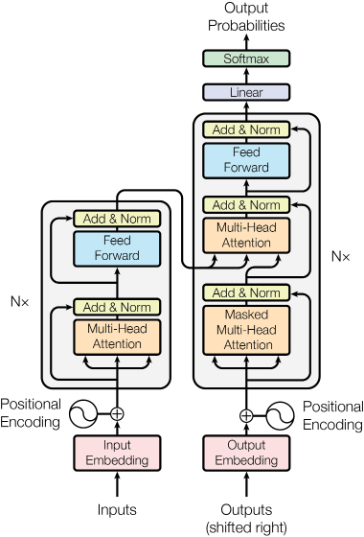
\includegraphics[width=0.4\textwidth]{figures/transformer_architecture.png}
    \caption[Transformer-Architektur]{Übersicht zur Transformer-Architektur nach~\textcite{vaswani2017attentionneed}}
    \label{fig:transformer_architecture}
\end{figure}

Der Encoder, welcher die linke Hälfte in Abbildung~\ref{fig:transformer_architecture} darstellt, erzeugt aus einer Input-Sequenz bestehend aus Symbolen eine numerische Repräsentation. Der Decoder, in Abbildung~\ref{fig:transformer_architecture} auf der rechten Seite, nutzt diesen numerischen Repräsentationsvektor, um die einzelnen Elemente einer symbolischen Output-Sequenz nach und nach zu generieren. Zu erwähnen ist dabei die Autoregressivität des Modells, was bedeutet, dass es bei der Generierung des nächsten Elements die bereits erzeugten Elemente als zusätzlichen Input nutzt \autocite{vaswani2017attentionneed}. Der Encoder entwickelt also ein Sprachverständnis im mathematischen Sinn und der Decoder ist für die Textgenerierung trainiert. Sprachmodelle können dann in Encoder-only-, Decoder-only- und Encoder-Decoder-Architekturen, die Encoder und Decoder kombinieren, unterteilt werden \autocite{huggingFaceTransformer}. Zu den „attention mechanisms“, die die Transformer-Architektur nutzt gehört die „self-attention“ als Kernprinzip. Dabei wird das Modell angewiesen, die Repräsentation jedes Worts in einem übergebenen Satz im Kontext der anderen Wörter zu sehen und diesen anderen Wörtern mehr oder weniger Aufmerksamkeit zu schenken. So werden auch Wörter, die in einem Satz weiter auseinander liegen zueinander in Beziehung gesetzt. Mit dieser neu geschaffenen Architektur konnten auf dem „WMT 2014 English-to-German translation task“ bessere Ergebnisse als mit allen bis dato getesteten Modellen und dazu noch deutlich geringere Trainingskosten im Sinne von Rechenoperationen und Trainingszeit, aufgrund der nun erreichten parallelen Verarbeitung, erreicht werden \autocite{vaswani2017attentionneed}. \\
Die Transformer-Architektur stellt jedoch lediglich das strukturelle Fundament dar, auf dem große Sprachmodelle arbeiten. Es bedarf zusätzlich eines Pre-trainings, damit die Modelle ihr volles Potenzial ausschöpfen können. Dazu werden enorme Datenmengen verwendet, um die initialen Modellparameter zu trainieren und dem Modell ein Verständnis der grundlegenden Sprachmuster beizubringen. Die Datenqualität und -diversität sind essenziell für die Modellperformance, weshalb eine umfassende Datensammlung, sowie eine äußerst sorgfältige Vorverarbeitung erfolgen muss. Diese Daten werden dann auf Tokens reduziert und in einzelnen Batches zum verteilten Training der Modelle genutzt. Für das Pre-training der großen Sprachmodelle wird nicht nur eine enorme Rechenkapazität benötigt, es müssen auch Entwickler mit einer großen Expertise vorhanden sein, damit ressourcenschonend und mit dem bestmöglichen Ergebnis gearbeitet werden kann.
Zusätzlich zum Pre-training verwenden viele Hersteller von LLMs Fine-tuning, um ihre Modelle von einem allgemeinen Zustand hin zur Verarbeitung spezifischer Aufgaben zu trainieren. Dabei wird dem Modell typischerweise kein neues Wissen zugeführt, sondern dessen bestehende Fähigkeiten werden weiter verbessert. Die gängigste Form ist das Instruction-Tuning, womit das Modell befähigt wird, Anweisungen, die es in natürlicher Sprache erhält, auszuführen. Das Modell lernt quasi durch beobachtendes Lernen anhand von Beispielen oder Demonstrationen, wie eine bestimmte Aufgabe zu erledigen ist. Dazu wird nur ein Bruchteil der Daten benötigt, die für das initiale Pre-training benötigt wurden, um zufriedenstellende Ergebnisse zu erreichen.
Darüber hinaus wird ein sogenanntes „human alignment“ durchgeführt, was primär über „Reinforcement Learning from Human Feedback“ (RLHF) erfolgt. Dabei wird ein Belohnungsmodell mit dem Feedback von Menschen trainiert, die verschiedene Antworten des generativen Modells vergleichen und bewerten. Das Belohnungsmodell nutzt das Feedback, um dem generativen Modell bei der Bewertung der Qualität seines Outputs zu helfen.
Sind diese drei Schritte absolviert, hat das Modell die Fähigkeit entwickelt komplexe Aufgaben zu erledigen und mit einem Endnutzer zu interagieren und dessen Anweisungen zu befolgen \autocite{Zhao_Zhou_Li_Tang_Wen_2026}. \\
Die praktische Evolution von LLMs lässt sich mit Blick auf ihre rasante technologische Entwicklung in den vergangenen Jahren verstehen \textcolor{red}{(Dieser Satz überzeugt mich nicht. Entweder komplett raus oder umschreiben.)}. Nachdem im Jahr 2017 der Grundstein gelegt wurde, zeigte sich im Jahr 2018 mit der Veröffentlichung von GPT erstmals das Potenzial eines autoregressiven Modells, das immense Fähigkeiten in der Generierung synthetischer Texte besaß \autocite{kehkashan2025}. Bereits ein Jahr später erschien GPT-2, das gezeigt hat, wie gut große Sprachmodelle bei der Absolvierung einer Reihe verschiedener Aufgaben ohne eine explizite Überwachung abschneiden können \autocite{radford2019language}. Doch erst die Veröffentlichung von GPT-3 und ChatGPT, das GPT-3.5 nutzt, ein für den Einsatz als Chatbot spezialisiertes GPT-3, schaffte es, dank der einfachen Nutzeroberfläche, dass große Sprachmodelle in der Mitte der Bevölkerung ankamen \autocite{openai2022}. Diese Modelle zeichneten sich bereits durch eine sehr hohe Parameterzahl aus und wurden auf deutlich größeren Datensätzen trainiert, was zur Folge hatte, dass immer natürlicher wirkende Texte generiert werden konnten. Mit GPT-4 folgte das erste Modell, das Multimodalität implementierte und die Generierung und das Verständnis nicht mehr nur auf Text beschränkte \autocite{Proehl_Mohrhardt_Foerster_Putzier_Zarnekow_2024}. Neben OpenAI und deren GPT-Familie etablierten sich auch andere Player innerhalb des LLM-Kosmos, wie oben kurz erwähnt. Entwickler von Meta veröffentlichten im Jahr 2023 mit der ersten LLaMA-Serie Open-Source-LLMs, die ausschließlich auf öffentlich verfügbaren Datensätzen trainiert wurden und deren Quellcode öffentlich einsehbar ist und mit den State-of-the-Art-Modellen dieser Zeit konkurrenzfähig ist \autocite{touvron2023llamaopenefficientfoundation}. Eine Weiterentwicklung dieser Modelle, die Version 3, wurde im Jahr 2024 vorgestellt und agierte dabei auf einem Niveau mit GPT-4 von OpenAI, hinsichtlich der Verarbeitung von Text, Bild, Video und gesprochener Sprache. Zusätzlich wurde über ein Post-Training erreicht, dass die Modelle auch Anweisungen folgen \autocite{grattafiori2024llama3herdmodels}.
Dieser kurze Abriss der raschen Entwicklung generativer Sprachmodelle zeigt die Schwierigkeit mit der erkennende Verfahren konfrontiert sind. Das ganze lässt sich als ein Wettrüsten sehen, „as each leap in model scale has corresponded with qualitative improvements in generation capabilities that challenge existing detection methods [\dots], coinciding with significantly more human-like text generation that required entirely new detection paradigms“ \autocite{kehkashan2025}. Aus diesem Grund stellt sich auch die Frage, inwieweit heutiger KI-Text mit Detektoren erkannt werden kann, die zur Erkennung deutlich älterer generativer Modelle entwickelt wurden.


\section{Charakteristika KI-generierter Texte}
\label{sec:charakteristika_ki}
Guo et al. \autocite{guo2023closechatgpthumanexperts}, haben im Rahmen der Entwicklung eines Detektors eine Analyse bezüglich der charakteristischen Eigenschaften von KI-generiertem und von Menschen verfassten Text durchgeführt. Freiwillige sollten anhand des Datensatzes, der später zum Training des Detektors verwendet wurde, Antworten von ChatGPT und von echten Menschen vergleichen und die jeweiligen Merkmale zusammenfassen. Zunächst fällt auf, dass Antworten von ChatGPT einer klaren Struktur folgen. Dabei wird zunächst noch einmal der Kern der Frage bzw. der Aufgabe wiederholt, gefolgt von einer Schritt-für-Schritt-Erklärung oder -Anleitung und abschließend wird eine Zusammenfassung bereitgestellt. Die KI-generierten Antworten sind häufig lang und weisen einen hohen Detailgrad auf, was Guo et al. \autocite{guo2023closechatgpthumanexperts} auf das RLHF zurückführen. ChatGPT ist in seinen Antworten oft darauf bedacht bei sensiblen Themen eine neutrale Position einzunehmen \textcolor{red}{(Hier vielleicht noch Quelle, die diese Neutralität aufgreift?)}. Zudem antwortete ChatGPT in den von Guo et al. \autocite{guo2023closechatgpthumanexperts} durchgeführten Analysen nicht auf Fragen, deren Antwort es glaubt nicht zu wissen \textcolor{red}{(Vielleicht ein Gegenbeispiel dazu?)}. Auch hier führen die Forscher an, dass dies durch RLHF erreicht wurde, um die Grenzen des Modellwissens automatisch zu erkennen. Ein großes Problem, was große Sprachmodelle, alleine aufgrund ihrer Architektur, haben, sind sogenannte „Halluzinationen“, also die Wiedergabe von entweder falschen oder gänzlich erfundenen Informationen mit der Überzeugung, dass es sich dabei um die Wahrheit handelt. Diesen Befund konnten \autocite{guo2023closechatgpthumanexperts} auch quantifizieren/bestätigen. Guo et al. \autocite{guo2023closechatgpthumanexperts} fanden heraus, dass bei Fragen, auf die es bisher keine Antwort gibt, dennoch eine Antwort mit erfundenen Fakten von ChatGPT zurückgegeben wird, nur um die Frage zu beantworten. \\
Im Vergleich zu Antworten von ChatGPT, weisen menschliche Antworten keine strenge Konzentration auf die eigentliche Frage auf. Menschen haben ein tiefergehendes Verständnis von Sprache und erkennen versteckte Bedeutungen mittels Menschenverstand und ihrem angehäuften Wissen und verlassen sich nicht ausschließlich auf das geschriebene Wort. Einerseits verwendet ChatGPT eine deutlich neutralere und ausgeglichenere Sprache, andererseits sind Menschen besser im Belegen ihrer Aussagen hinsichtlich der Verwendung überprüfbarer Quellen in einem wissenschaftlichen, rechtlichen oder technischen Kontext \textcolor{red}{(Sollte sich mittlerweile deutlich geändert haben, siehe Gemini AI Overview usw.; dazu vielleicht aktuelle Quelle)}. Menschen benutzen deutlich mehr Umgangssprache, Slang, Ironie und auch Methapern, während ChatGPT auf eine formale Sprache setzt \textcolor{red}{(Auch hier mittlerweile anders, je nachdem wie die "Persönlichkeit" der KI vom Nutzer oder den Entwicklern festgelegt wurde. Hierzu vielleicht auch neuere Quelle)}. Ein auffälliger Unterschied ist auch die deutlich andere Verwendung von Interpunktion durch Menschen. Menschen kommunizieren ihre Gefühle häufig über die Wiederholung von Satzzeichen oder Ellipsen und nutzen Klammern um bestimmte Dinge zu ergänzen. Hier setzt sich auch der strukturierte Aufbau von ChatGPT-Antworten fort, was sich in der Verwendung von Formulierungen wie „Firstly,...,Secondly,...,Finally“ widerspiegelt. \autocite{guo2023closechatgpthumanexperts}. \\
Ter\v{c}on und Dobrovoljc \autocite{tercon2025linguisticcharacteristicsaigeneratedtext} kommen nach einer systematischen Untersuchung zu dem Schluss, dass es hinsichtlich Vokabular, Satzlänge und Stil mehr oder weniger deutliche Unterschiede zwischen den verschiedenen Modellen auf dem Markt gibt \textcolor{red}{(Soll ich hier noch genauer drauf eingehen?, S.13-14)}. Auch hinsichtlich des Kontextes, in dem der Text von einem LLM verfasst wurde, gibt es Abweichungen zwischen verschiedenen Genres. Wissenschaftliche Texte, die KI-generiert wurden, weisen oft weniger erzählende Elemente auf und verwenden mehr überzeugend wollende Sprache, als von Menschen verfasste Texte. Dies entspricht auch dem oben geschilderten Befund von Guo et al. \autocite{guo2023closechatgpthumanexperts}. In Bezug auf Konversationen nutzen Sprachmodelle eher abstraktere Formulierungen als Menschen und wirken weniger involviert in die Thematik.  Bezüglich der verwendeten Sprache konnten bei japanischen generierten Texten häufiger Grammatikfehler und fehlerhafte Schreibsysteme festgestellt werden. Zudem gibt es Anzeichen für Unterschiede in der Erkennungswahrscheinlichkeit, wenn dem zu erkennenden generierenden Sprachmodell nicht nur der Titel, sondern auch ein entsprechender von Menschen verfasster Textausschnitt zur Verfügung gestellt wird. In diesem Fall erzeugt das Modell einen, linguistisch gesehen, „menschlicheren“ Output \textcolor{red}{(Könnte eventuell auch für mich relevant sein, da ich ja die ersten 300 Zeichen des Textes mitgebe.)}. \\
Zusätzlich zur oben beschriebenen Analyse haben Guo et al. \autocite{guo2023closechatgpthumanexperts} auch eine linguistische Untersuchung des in der Detektorentwicklung verwendeten Datensatzes vorgenommen. Im Hinblick auf das Vokabular zeichnen sich von Menschen verfasste Texte durch eine größere Vokabulargröße und „Dichte“ aus, als dies bei künstlich generierten Texten der Fall ist. „Dichte“ definieren die Forscher dabei als Maßzahl dafür, wie viele verschiedene Wörter im Verhältnis zur Länge des Textes genutzt werden. Umso höher die Dichte eines Textes, desto mehr verschiedene Wörter werden bei der gleichen Textlänge verwendet und desto diverser ist das Vokabular \autocite{guo2023closechatgpthumanexperts}. Auch \autocite{tercon2025linguisticcharacteristicsaigeneratedtext} schlussfolgern aus der aktuellen Forschung eine niedrigere lexikalische Diversität in KI-generierten Texten, was sich in einem weniger diversen Wortschatz äußert. Hinsichtlich des verwendeten Vokabulars zeigen sich in KI-Texten weniger häufig Wörter, die mit bestimmten negativen Gefühlen assoziiert sind oder Ausdrücke von Aggressivität und Unhöflichkeit \autocite{tercon2025linguisticcharacteristicsaigeneratedtext}. Bezüglich der durchschnittlichen Antwortlänge sind von ChatGPT erzeugte Texte in der Regel länger \autocite{guo2023closechatgpthumanexperts}. Zusätzlich weisen KI-generierte Texte eine niedrigere Variation an Satzlängen auf, als dies bei Menschen der Fall ist \autocite{tercon2025linguisticcharacteristicsaigeneratedtext}. Allerdings gibt es laut Ter\v{c}on und Dobrovoljc in der Forschung keinen Konsens darüber, ob es einen Unterschied in der durchschnittlich verwendeten Satzlänge zwischen KI- und Menschen-Text gibt \autocite{tercon2025linguisticcharacteristicsaigeneratedtext}. Betrachtet man die Verwendung bestimmter Wortarten, fällt auf, dass ChatGPT mehr Nomen, Verben, Determinativa, Adjektive, Hilfsverben, koordinierende Konjunktion und Partikel nutzt, als Menschen. Seltener als von Menschen werden Adverben und Interpunktion verwendet. Deutliche Unterschiede sind im Sentiment der Antworten von Menschen und von ChatGPT quantifizierbar. ChatGPT drückt sich deutlich häufiger neutral aus und Menschen kommunizieren signifikant häufiger negative Gefühle \autocite{guo2023closechatgpthumanexperts}. Ter\v{c}on und Dobrovoljc fassen zusammen, dass es vom Kontext abhängig ist, ob KI-generierter Text emotionaler als von Menschen verfasster Text ist, wobei sie übereinstimmen, dass ersterer häufiger eine neutrale Stimmung transportiert.



When comparing question answering texts in Chinese and English, Guo et al. (2023) note that the
human-produced answers are shorter and contain a larger vocabulary size, and that this tendency is more
pronounced in Chinese texts than in English. However, the tendency can be found in both languages to
some extent. \autocite{tercon2025linguisticcharacteristicsaigeneratedtext} \textcolor{red}{(In Guo suchen und einbauen)}

\section{Verfahren zur Erkennung KI-generierter Texte}
Wie bereits dargestellt, geht der rasante Fortschritt generativer Sprachmodelle unmittelbar mit ihrer Fähigkeit zu zunehmend authentisch menschlich klingenden Texten einher. Daher fällt einer zuverlässigen Identifikation synthetischer Texte immer mehr Bedeutung zu. Nicht umsonst etablierte sich die Erkennung KI-generierter Texte zu einem eigenständigen Forschungsfeld, innerhalb dessen verschiedene methodische Ansätze verankert sind \autocite{kehkashan2025}. Dabei unterscheiden Kehkashan et al. \autocite{kehkashan2025} zwischen statistischen und linguistischen Ansätzen, Machine-Learning-basierten Verfahren, Zero-Shot und modellspezifischen Methoden, sowie Boundary Detection und der Teiltextanalyse.

\subsection{Statistische und linguistische Verfahren}
Statistische Detektionsverfahren legen das Hauptaugenmerk auf sprachliche und stilistische Merkmale in einem Text. Dabei werden gängige Methoden der Computerlinguistik angewandt, um eben diese stilistischen und sprachlichen Muster zu erkennen. Die Erkennung dieser Muster hilft dabei, von Menschen geschriebene Texte systematisch von künstlich generierten Texten abzugrenzen \autocite{kehkashan2025}. Dabei sind stilistische und sprachliche Muster als quantitativ erfassbare Merkmale in einem Text zu verstehen, anhand derer verschiedene Detektionsmodelle charakteristische Unterschiede zwischen Texten erlernen können \autocite{Proehl_Mohrhardt_Foerster_Putzier_Zarnekow_2024}. In diesem Kontext stellt die N-gram-Analyse ein grundlegendes historisches Verfahren dar, um maschinell erzeugte Texte zu erkennen. Dabei wird zunächst die Verteilung von Wort- oder Zeichensequenzen untersucht, um diese dann mit der erwarteten Verteilung in von Menschen verfassten Texten zu vergleichen. Mit N-grams können sowohl ein auffälliges Vokabular (1-gram), als auch Muster in Sequenzen erfasst werden. So werden ungewöhnliche Wörter oder Wortkombinationen aus einem Text herausgearbeitet und anhand ihrer Verteilung kann erkannt werden, ob es sich um KI-generierten oder von Menschen verfassten Text handelt. Eine Limitation dieser Methode ist die Schwäche den Output der modernen LLMs korrekt zu klassifizieren \autocite{kehkashan2025}.
Neben diesem Verfahren gibt es die Möglichkeit die sogenannte „Perplexity“ als Kennzahl für die Klassifikation von Text zu nutzen. Sie gibt an, wie überrascht oder „perplex“ ein Modell ist, wenn es den nächsten generierten Token sieht. Diesem Verfahren liegt die Annahme zugrunde, dass von Menschen verfasste Texte nicht einem Muster der Vorhersagbarkeit folgen bzw. Menschen nicht immer die statistisch wahrscheinlichste nächste Sequenz wählen. Bei Verfahren, die diese Metrik nutzen, „wird für jeden Token die Wahrscheinlichkeit bestimmt, dass er als nächster Token generiert wird“ \autocite{Proehl_Mohrhardt_Foerster_Putzier_Zarnekow_2024}. Text, der von einem Sprachmodell generiert wurde, basiert eben genau darauf, den wahrscheinlichsten nächsten Token zu generieren \autocite{Proehl_Mohrhardt_Foerster_Putzier_Zarnekow_2024}. So lassen sich Texte bzw. Sequenzen, die eine niedrige Perplexität aufweisen, als wahrscheinlich KI-generiert identifizieren. Als weitere Maßzahl hat sich die sogenannte „Burstiness“ etabliert. Sie beschreibt die Muster, die in der Wortwahl und Variation des Vokabulars beobachtet werden können \autocite{chakraborty2023counterturingtestct2}. Ähnlich wie auch bei der „Perplexity“ ist hier die Annahme, dass LLMs aufgrund ihrer Architektur, den durchschnittlichsten Schreibstil anhand der Trainingsdaten gelernt haben. Sprachmodelle verwenden also in der Regel Wörter, die eher häufiger vorkommen, da diese wahrscheinlicher auf das vorhergehende Wort folgen. Menschen unterscheiden sich eher in ihrem Vokabular, ihrer Vokabulargröße und schreiben häufiger unterschiedlich lange Sätze und haben somit unterschiedliche Schreibstile. Die „Burstiness“ ist also ein Maß dafür, wie sehr sich der Schreibstil des generierten Textes von dem üblichen „menschlichen“ Schreibstil unterscheidet \autocite{Proehl_Mohrhardt_Foerster_Putzier_Zarnekow_2024}.

\subsection{Machine-Learning-basierte Verfahren}
Zu den Machine-Learning-basierten Verfahren die zur Erkennung von KI-generiertem Text genutzt werden, zählen zwar auch klassische Klassifikatoren, wie Support Vector Machines und Random Forests, aber in der jüngeren Vergangenheit haben sich vor allem Künstliche Neuronale Netzwerke als ergiebig herausgestellt. Sie haben den Vorteil, dass sie eine deutlich höhere Leistungsfähigkeit aufweisen, wobei dies zur Folge hat, dass sie auf großen Datenmengen trainiert werden müssen und dafür viel Rechenkapazität benötigt wird. In diesem Kontext sind die Transformer-basierten Detektoren der neueste Stand der Technik und vor allem vortrainierte Modelle, die mittels Fine-Tuning auf die Erkennung von KI-generiertem Text spezialisiert trainiert wurden. Dabei handelt es sich in der Regel um binäre Klassifikatoren, die auf der Encoder-Architektur aufbauen, und somit ein ausgeprägtes Textverständnis aufweisen, wie in Kapitel~\ref{sec:LLMintro} beschrieben \autocite{kehkashan2025}. Die Modelle werden beim Fine-Tuning darauf trainiert selbstständig die Muster zu erkennen, die KI-generierten Text von menschlich verfasstem Text unterscheiden \textcolor{red}{(Weiß nicht, was hier als Quelle geeignet ist?)}. Dazu werden gelabelte Daten benötigt, die sowohl generierten Text, als auch maschinell-erzeugten Text enthalten, allerdings in einem weitaus geringeren Maßstab, als dies bei einem nicht-vortrainierten Modell der Fall wäre (siehe Kapitel~\ref{sec:LLMintro}). Da allerdings ein immenser Datensatz notwendig wäre, um alle Sprachen, Schreibstile, Kontexte und auch Eigenheiten der generierenden Modelle zu berücksichtigen, bietet sich das Training eines Modells für ein spezifisches Thema oder Rahmen an \autocite{Proehl_Mohrhardt_Foerster_Putzier_Zarnekow_2024}. Wissenschaftliche Arbeiten unterliegen anderen Formalitäten/Gegebenheiten als Beiträge auf Social Media. Entwickler von verschiedenen Detektormodellen versuchen zwar ein möglichst breites Spektrum an möglichen Eingabesequenzen abzubilden, in der Praxis kann es aber dennoch oft zu Abweichungen vom Gelernten kommen. Deshalb ist die Klassifikationsleistung stark abhängig von der Ähnlichkeit der Trainingsdaten und den zu klassifizierenden Texten. \textcolor{red}{(Hier noch Zitat und Verweis auf Kapitel 2.5?)}. Modelle, die diesen Ansatz nutzen, sind der in dieser Arbeit verwendete RoBERTa OpenAI Detector und der ChatGPT Detector RoBERTa (siehe Kapitel~\ref{subsec:robertaopenai} bzw. \ref{subsec:chatgptdetectorroberta}).

\subsection{Zero-Shot-Verfahren}
Die sogenannten Zero-Shot-Verfahren kommen ohne ein vorheriges Training auf einem Beispieldatensatz oder ein Fine-Tuning aus. Die Modelle aus dieser Verfahrensklasse werden direkt auf den zu klassifizierenden Text angewandt und benötigen daneben nur den Zugang zu den zu testenden generierenden Modellen \autocite{Proehl_Mohrhardt_Foerster_Putzier_Zarnekow_2024}. Dabei gibt es kein striktes „Drehbuch“, wie die Erkennung konkret umgesetzt werden muss und so haben sich innerhalb dieses Verfahrens verschiedene Ansätze entwickelt, die gemeinsam haben, dass sie die von Sprachmodellen genutzten Mechanismen der Wahrscheinlichkeit verwenden \autocite{kehkashan2025}. So nutzen Mitchell et al. \autocite{mitchell2023detectgptzeroshotmachinegeneratedtext} mit DetectGPT „only log probabilities computed by the model of interest and random perturbations of the passage from another generic pre-trained language model“. Dem Modell liegt die Annahme zugrunde, dass Ausgaben von einem generativen Quell-Sprachmodell üblicherweise in Bereichen mit negativer Krümmung der logarithmischen Wahrscheinlichkeitsfunktionen des Modells liegen. Von Menschen verfasste Texte liegen eher nicht in diesen Bereichen mit eindeutig negativer Krümmung und semantisch ähnliche Texte von Menschen können eine höhere oder auch niedrigere logarithmische Wahrscheinlichkeit haben. Um Perturbationen des Originaltextes zu erzeugen, nutzen die Forscher ein Sprachmodell, das diese Texte in semantisch ähnliche Versionen umformuliert. Dabei können ganze Wörter ersetzt werden, die aber dennoch eine semantische Ähnlichkeit aufweisen, oder bestimmte Sequenzen des Textes komplett gestrichen werden, ohne dabei die grundlegende Bedeutung des Satzes zu verändern. Je näher die logarithmierten Wahrscheinlichkeiten des Ursprungstexts und die durchschnittlichen logarithmierten Wahrscheinlichkeiten der Perturbationen beieinander liegen, desto eher ist der Text von Menschen verfasst \autocite{mitchell2023detectgptzeroshotmachinegeneratedtext}. Ein weiteres prominentes Beispiel für ein Zero-Shot-Verfahren ist das Binoculars Framework, was im Abschnitt~\ref{subsec:binoculars} detaillierter betrachtet wird. Eine Schwäche dieser Verfahren ist, dass oft bekannt sein muss, welche logarithmische Wahrscheinlichkeitsfunktion dem zu erkennenden generierenden Modell zugrunde liegt. Viele Entwickler von LLMs stellen diese Möglichkeit nicht zur Verfügung \autocite{SUN2025129829}.

\subsection{Adversarial Learning}
Die Idee des sogenannten „Adversarial Learning“ stammt von Goodfellow et al. \autocite{goodfellow2014generativeadversarialnetworks}. Dabei sollen gleichzeitig zwei verschiedene Modelle trainiert werden, ein  „discriminator“ und ein „generator“. Diese stehen in einem Wettbewerb zueinander, wobei das diskriminative Modell lernen soll, den Output des generierenden Modells richtig zu klassifizieren. Der „generator“ hat zur Aufgabe den „discriminator“ mit möglichst echt wirkenden Inhalten zu täuschen. Beide Modelle werden im Zuge dieses Wettbewerbs dazu gezwungen, ihre jeweiligen Methoden bei der Generierung bzw. Unterscheidung immer weiter zu verbessern, bis auf beiden Seiten keine Optimierung mehr möglich ist. Dieses Konzept haben Hu et al. \autocite{hu2023radar} auf die Erkennung von KI-generiertem Text übertragen. Dort werden ein Paraphrasierer und ein Detektor in Konkurrenz zueinander gestellt. Die Funktionsweise dieses Modells wird in Kapitel~\ref{subsec:radar} näher erläutert.

\section{Die untersuchten Detektoren}
Im Rahmen dieser Bachelorarbeit sollen vier verschiedene Detektoren zur Erkennung von KI-generiertem Text evaluiert werden, welche im Folgenden beschrieben werden.

\subsection{RoBERTa OpenAI Detector}
\label{subsec:robertaopenai}
Die Modelle RoBERTa Base OpenAI Detector bzw. RoBERTa Large OpenAI Detector waren einer der ersten Versuche Text, der durch Large Language Models generiert wurde, zu erkennen. Grundlage dieser beiden Modelle ist RoBERTa \autocite{RoBERTa2019}, was wiederum eine verbesserte Variante des BERT-Modells ist. Diese Modelle verwenden die Encoder-Architektur und sind damit lediglich in der Lage Text zu verstehen und nicht zur Textgenerierung fähig. Mittels Fine-Tuning auf einem Datensatz, der aus von Menschen generiertem Text und Output von GPT-2 besteht, wurde RoBERTa auf die Erkennung von
KI-generierten Texten angepasst. Der von Menschen generierte Text stammt aus dem WebText-Datensatz, welcher auch für das initiale Training von GPT-2 verwendet wurde \autocite{RoBERTaDetector2019}. Gemessen am Volumen ist Google die größte Quelle für den WebText-Datensatz, wobei Reddit nicht als solches unter den 1.000 häufigsten Datenquellen zu finden ist \autocite{gpt2dataset}. Für den GPT-2-Output wurden vier verschiedene Varianten des Modells mit einer unterschiedlichen Anzahl an Parametern (124 Millionen, 355 Millionen, 774 Millionen und 1,5 Milliarden) verwendet.\\
Solaiman et al. \autocite{RoBERTaDetector2019} kommen zu dem Ergebnis, dass mit diesem Modell KI-generierter Text mit einer Genauigkeit von ungefähr 95 \% erkannt wird. Die Genauigkeit wurde dabei anhand von 5.000 Stichproben aus dem WebText-Datensatz und 5.000 mit GPT-2 generierten Texten, die nicht im Training der GPT-2-Modelle verwendet wurden, mit einer Länge von jeweils 510 Token gemessen. \\
\autocite{Ibrahim2023UsingAD} untersuchte die Leistung des RoBERTa Large OpenAI Detectors im Kontext von Erwachsenenbildung. Bei den von Menschen generierten Texten handelt es sich um eine Zufallsstichprobe von 120 englischen Essays, die von nicht-muttersprachlichen Studenten an einer amerikanischen Universität in Kuwait im Rahmen eines Projekts zum Thema „Forschungsargumentation“ verfasst wurden. Durch eine zeitliche Beschränkung auf Essays, die vor der Veröffentlichung von ChatGPT verfasst wurden, sollte sichergestellt werden, dass die eingereichten Essays nicht mithilfe von Künstlicher Intelligenz generiert wurden. Um die KI-generierte Stichprobe zu erzeugen, wurde ChatGPT 3.5 genutzt, wobei als Prompt die Projektbeschreibung des Kurses übergeben wurden, ebenso wie eine Einschränkung auf Themen, die auch in den von Menschen verfassten Essays vorkamen. Getestet wurden zwei Modelle, die auf dem RoBERTa OpenAI Detector basieren, mit dem Ergebnis, dass das vom Forscher verwendete Modell GPT-2 Output Detector Demo mit einer Genauigkeit von 89,2 \% zwischen von Menschen geschriebenen und von KI generierten Texten unterscheiden kann.\\
Die primäre Limitation des Modells liegt darin, dass es darauf trainiert worden ist, Output von GPT-2 zu erkennen. Neuere, fortgeschrittenere Modelle sind seitdem auf dem Markt und erschweren die Detektion von KI-generiertem Text durch den RoBERTa OpenAI Detector vermutlich deutlich. Eine weitere Einschränkung, die OpenAI macht, ist, dass der Output von größeren Modellen schwerer zu klassifizieren ist und sich dieser Trend mit fortschreitender Vergrößerung der Modelle weiter fortsetzen wird. Außerdem gehen die Forscher von OpenAI davon aus, dass die 95 \%-ige Genauigkeit nicht ausreicht, um den Detektor als Standalone-Lösung zu verwenden und es ergänzende Methoden wie metadaten-basierte Ansätze, menschliche Einschätzung und öffentliche Bildung braucht \autocite{openai2019}. Des Weiteren fanden Forscher der Universität Stanford heraus, dass der RoBERTa OpenAI Detector über die Hälfte der Essays von Nicht-Muttersprachlern fälschlicherweise als KI-generiert erkannt hat, während Essays von US-amerikanischen Achtklässlern nur in 9 \% der Fälle als False Positive klassifiziert wurde \autocite{liang2023gptdetectorsbiasednonnative}. Allerdings beschreiben die Entwickler von OpenAI selbst in der Model Card des Detektors, dass davon abgeraten wird, den Detektor zu benutzen, um Studenten des wissenschaftlichen Fehlverhaltens zu beschuldigen, aufgrund der eventuell ungenauen Ergebnisse im Falle von durch ChatGPT generierten Inputs \autocite{modelcardRoBERTaDetector}.  \\
Der RoBERTa Large OpenAI Detector soll im Rahmen dieser Bachelorarbeit als Baseline fungieren, da er im Kontext des frühen Entwicklungsstadiums der LLMs veröffentlicht wurde. Außerdem kann so überprüft werden, ob der Bias gegen Nicht-Muttersprachler, angesichts der Reddit-Nutzerschaft auch im von mir durchgeführten Experiment fortbesteht.

\subsection{ChatGPT Detector RoBERTa}
\label{subsec:chatgptdetectorroberta}
Der ChatGPT Detector RoBERTa basiert ebenfalls auf dem Modell RoBERTa und nutzt Fine-Tuning, um die Erkennungsfähigkeit des Modells zu verbessern. Zum Fine-Tuning wurde ein Datensatz, bestehend aus mehreren Sub-Datensätzen, erzeugt. Die Datenquellen stammen aus den Domänen Soziale Medien, Medizin, Finanzen und Wikipedia. Sie umfassen den Subreddit „ELI5“, den Microsoft Research WikiQA Corpus, Wikipedia, den Medical Dialogue Datensatz und den FiQA Datensatz, wobei der größte Anteil auf den Subreddit „ELI5“ entfällt. Die Sub-Datensätze haben gemeinsam, dass sie Fragen als Ausgangspunkt haben, zu denen von Menschen verfasste Antworten verfügbar sind. Um KI-generierte Antworten auf diese Fragen für den Datensatz zu sammeln, wurden ebendiese Fragen als Prompt für ChatGPT verwendet. Die Forscher verwenden zur Evaluation insgesamt sechs verschiedene Trainings- und Testdatensätze. Zum einen wird der „rohe“ Datensatz verwendet, der dann gefiltert wird, indem Wörter die, basierend auf vorhergehenden Analysen, einen Hinweis auf den Ursprung des Textes geben könnten und somit die Differenzierung vereinfachen könnten, entfernt werden. Die so erzeugten beiden Sets werden dann jeweils in Sätze getrennt, um zwei weitere Datensätze zu erzeugen, mit denen untersucht werden soll, ob die Länge des zu klassifizierenden Textes einen Einfluss auf die Erkennung hat. Außerdem werden jeweils Versionen des „rohen“ und des gefilterten Datensatzes mit einer Mischung aus Sätzen und den gesamten Texten erzeugt. Das Modell wird dann auf all diesen Datensätzen trainiert und getestet. Im Schnitt kommen die Forscher auf einen F1-Score von 98,78 \%  \textcolor{red}{(Vielleicht Grafik aus Paper nutzen zum besseren Verständnis?)}. Die Autoren merken an, dass die Menge der genutzten Daten zwar sehr hoch ist, aber nicht ausreichend. Ebenso ist die Menge der Daten in den jeweiligen Sub-Datensätzen ungleich verteilt, weshalb in ihren Augen nicht genügend Varianz hinsichtlich verschiedener Stile und Sprachen vorhanden ist. Außerdem beziehen sich alle Ergebnisse und Schlussfolgerungen auf ChatGPT-Antworten, die ohne einen speziellen Prompt erzeugt worden sind. Prompts, die z. B. einen speziellen Schreibstil fordern, könnten den Detektor umgehen \autocite{guo2023closechatgpthumanexperts}. \\
In \autocite{he2024mgtbenchbenchmarkingmachinegeneratedtext} wurde der ChatGPT Detector RoBERTa noch einmal validiert und mit anderen Detektoren verglichen. Dazu wurden drei unterschiedliche Datensätze genutzt, die von \autocite{verma2024ghostbusterdetectingtextghostwritten} erzeugt worden sind. Grundlage dieser Datensätze waren von Menschen in Schulen und Universitäten verfasste Essays, Geschichten aus dem Subreddit „r/WritingPrompts“ und (Nachrichten-) Artikeln von Journalisten der Nachrichtenagentur Reuters. Um dann die dazugehörigen „künstlichen“ Texte zu generieren, wurden entsprechende Prompts aus den realen Daten abgeleitet und als Prompt für verschiedene generierende Modelle verwendet. Die Ergebnisse unterlagen starken Schwankungen, abhängig vom verwendeten Datensatz und dem generierenden Modell. Im Mittel ergab sich ein F1-Score von 61 \% auf dem Essay-Subdatensatz, 53,58 \% auf dem „r/WritingPrompts“-Subdatensatz und 68,05 \%, wobei bei ChatGLM als generierendem Modell durchgehend die besten Ergebnisse erzielt worden sind und bei Claude die schlechtesten.

\subsection{RADAR}
\label{subsec:radar}
RADAR wurde vor dem Hintergrund entwickelt, dass gängige Detektoren oft nicht robust gegenüber einer Paraphrasierung durch LLMs sind. Aus diesem Grund nutzten die Forscher „Adversarial Learning“, was meint, dass gleichzeitig ein Paraphrasierer und ein Detektor trainiert werden, was einen neuen Ansatz im Paradigma der KI-Erkennung darstellte. Der Paraphrasierer muss realistisch wirkenden Text erzeugen, um der Erkennung durch Detektoren zu entgehen und der Detektor muss die Erkennbarkeit von künstlich generiertem Text erhöhen. Die Datengrundlage für das Training bildete eine Stichprobe von 160.000 Dokumenten aus dem WebText-Datensatz. Die Forscher verwendeten dann acht verschiedene Zielmodelle, die ausgehend von den ersten 30 Tokens der Dokumente aus der Stichprobe, Textvervollständigung nutzen sollten, um künstliche Texte zu erzeugen. Zusätzlich wird dann ein weiteres Sprachmodell, GPT-3.5-Turbo, angewiesen den künstlichen Text zu paraphrasieren, um im Training den Detektor zu täuschen. Während des Trainings wird der Detektor, neben dem menschlichen Input, mit den KI-generierten Texten und dem Ergebnis des Paraphrasierers konfrontiert. Die Modellparameter des Detektors und des Paraphrasiers werden dabei solange aktualisiert, bis sich der Validation Loss der beiden im Wettbewerb stehenden Modelle stabilisiert. Evaluiert wird das Modell auf den Datensätzen Xsum, SQuAD, dem Subreddit „r/WritingPrompts“ und im Rahmen des TOEFL verfassten Essays. Diese Datensätze sollen den Detektor vor die Herausforderung stellen Fake News zu erkennen, Wissenschaftsbetrug zu verhindern, maschinell-generierte literarische Texte zu identifizieren und auf von Nicht-Muttersprachlern verfasste Texte zu reagieren. Der trainierte Detektor erreichte auf diesen Datensätzen im Schnitt über alle generierenden Zielmodelle hinweg einen AUROC-Score von 85,7 \%, wenn GPT-3.5-Turbo als Paraphrasierer genutzt wurde. Zwar geben die Forscher an, dass RADAR robuster gegenüber vergleichbaren Modellen im Hinblick auf Paraphrasierung ist, es aber dennoch dazu kommen kann, dass das Modell bei nativem KI-generiertem Text schlechter abschneidet als vergleichbare Modelle. Zudem weisen sie darauf hin, dass der von ihnen entwickelte Detektor auch falsche Vorhersagen liefern kann und nicht als einziger Indikator zur Erkennung von KI-generiertem Text verwendet werden soll \autocite{hu2023radar}.\\
Wird RADAR auf dem RAID-Datensatz evaluiert, erreicht es einen TPR@FPR=5\% von 65,6 \% und einen AUROC-Score von 81,9 \% \autocite{basani2026diversityboostsaigeneratedtext}. Basani und Chen \autocite{basani2026diversityboostsaigeneratedtext} testeten außerdem die Fähigkeit von RADAR auf unterschiedliche Attacken (u. a. Paraphrasierung und Rechtschreibfehler) basierend auf dem RAID-Datensatz zu reagieren. Im Ergebnis erreichte RADAR dabei einen TPR@FPR=5\% von 63,9 \% und einen AUROC-Score von 81,9 \%.

\subsection{Binoculars}
\label{subsec:binoculars}
Binoculars fällt in den Bereich der Zero-Shot-Detektoren, welche ohne Trainingsdaten auskommen. Diesem Modell liegt die Annahme zugrunde, dass sich moderne Sprachmodelle sehr in der verwendeten Architektur und Datenbasis zu ähnlichen Zeitpunkten ähneln. Zunächst werden zwei verschiedene Modelle betrachtet, ein „observer“-Modell und ein „performer“-Modell. Wichtig ist dabei, dass die Modelle den gleichen Tokenizer nutzen.
Um die Perplexität des „observer“-Modells zu berechnen, werden die logarithmischen Wahrscheinlichkeiten für jedes Wort in der Eingabesequenz ermittelt. Die Perplexität kann als Maß dafür verstanden werden, wie „überraschend“ jeder Token für das „observer“-Modell ist, wenn es den nächsten Token vorhersagt. Neben der Perplexität nutzen die Forscher eine weitere Metrik, die sie „cross-perplexity“ nennen, die misst, wie „überraschend“ die Vorhersagen für das nächste Token auf ein anderes Modell wirken. Der finale sogenannte „Binoculars score“ berechnet sich dann als Verhältnis zwischen der Perplexität des „observer“-Modells und der „cross-perplexity“ zwischen dem „observer“- und dem „performer“-Modell \autocite{hans2024spottingllmsbinocularszeroshot}. Zur Evaluierung nutzen die Forscher, ähnlich zu He et al. \autocite{he2024mgtbenchbenchmarkingmachinegeneratedtext} den von \autocite{verma2024ghostbusterdetectingtextghostwritten} erstellten Datensatz. Auf dem
Student Essay-Datensatz wird eine True Positive Rate von 97,6 \% bei einer False Positive Rate von 0,01 \% und ein F1-Score von 0.993 für die Erkennung von ChatGPT-generiertem Text erreicht. \\
Eine Limitation der Untersuchung ist, dass die Autoren aufgrund von GPU-Speicherbegrenzungen keine Modelle mit einem Parameterraum größer als 30 Milliarden nutzen konnten. Außerdem wurde nicht überprüft, wie Binoculars auf Attacken reagiert. Andere Textdomänen wie beispielsweise Quellcode wurden ebenfalls nicht betrachtet. \\
\autocite{basani2026diversityboostsaigeneratedtext} haben neben RADAR auch Binoculars auf dem RAID-Datensatz evaluiert und sind zu dem Ergebnis gekommen, dass Binoculars einen TPR@FPR=5\% von 79 \% und einen AUROC-Score von 84,4 \% erreicht. Steht das Modell unter Angriffen durch Paraphrasierung und ähnliches, wird ein TPR@FPR=5\% von 69,32 \% berichtet.

\section{Herausforderungen und Grenzen von KI-Detektoren}
\label{sec:herausforderungen_grenzen}
In den vorhergehenden Abschnitten sollte deutlich geworden sein, dass eine Erkennung von KI-generierten Texten aufgrund verschiedener Faktoren nicht trivial ist. Einige der Herausforderungen, mit denen Machine-Learning-Detektoren konfrontiert sind und wo ihre Grenzen liegen, soll im folgenden Kapitel dargestellt werden.
Ein großes Problem, das auch weiterhin besteht, stellt die Robustheit gegenüber von sogenannten Domain Shifts dar. Werden Detektoren auf einer bestimmten Textdomäne trainiert, sinkt deren Erkennungsleistung oft stark ab, wenn sie einer neuen Textdomäne ausgesetzt werden \autocite{pudasaini2026aigeneratedtextdetectionfails}. Zwar stehen alle Modelle vor diesem Problem, aber es gibt Anzeichen dafür, dass Detektoren, die mittels Fine-Tuning spezialisiert wurden, am besten über verschiedene Domänen hinweg generalisieren \autocite{baidya2026detectingmachinecomprehensivebenchmark}. Shen et al. \autocite{shen2026rethinkingaigeneratedtextdetection} kommen in diesem Zusammenhang zu dem Schluss, dass Detektor-Modelle häufig eine hohe Anzahl an False Positives deklarieren, was im AUROC nicht reflektiert wird, aber durch eine „low-FPR evaluation“ aufgedeckt werden kann und sehen „K-shot adaptation with a confidence-weighted ensemble“ als Lösung, um dieser zumindest teilweise entgegenzutreten. Diese Diskrepanz konnte auch in Kapitel~\ref{subsec:radar} und \ref{subsec:binoculars} festgestellt werden. \\
Eine weitere Herausforderung, die eng mit dem Domain Shift zusammenhängt, ist die Generalisierung über verschiedene generierende LLMs hinweg. Detektoren sind häufig nur auf einer Auswahl, der auf dem Markt zur Verfügung stehenden generativen Modelle trainiert worden und können so vor dem Problem stehen, die Outputs von neueren oder größeren Modellen zu erkennen. Beispielsweise ist der RoBERTa OpenAI Detector lediglich mit Outputs von GPT-2 trainiert worden (siehe Kapitel~\ref{subsec:robertaopenai}). Baidya et al. \autocite{baidya2026detectingmachinecomprehensivebenchmark} fanden heraus, dass eine „[c]ross-LLM generalization“ beobachtet werden kann, wenn für die Textdomäne kontrolliert wird. Methoden der Erklärbaren Künstlichen Intelligenz, wie Support Vector Machines, Random Forest oder die Logistische Regression haben deutliche Schwierigkeiten im Training nicht verwendete Sprachmodell zu erkennen \autocite{pudasaini2026aigeneratedtextdetectionfails}. Statistische Verfahren, die ausschließlich „Burstiness“ und „Perplexity“ zur Erkennung von KI-generiertem Text nutzen, geraten angesichts des Fortschritts in der LLM-Entwicklung, an ihre Grenzen Modelle der neueren Generationen verlässlich zu erkennen \autocite{chakraborty2023counterturingtestct2}. \\
Daneben müssen Detektoren auch Angriffen durch Paraphrasierung standhalten, da dies wohl der häufigste Fall beim Einsatz von generativen Sprachmodellen ist. Menschen nutzen den Output oft als Ausgangspunkt und nutzen Paraphrasierung, um entweder einer Detektion wissentlich zu entgehen oder um ihren eigenen Stil einfließen zu lassen. Krishna et al. \autocite{krishna2023paraphrasingevadesdetectorsaigenerated} entwickelten ein paraphrasierendes Modell mit dem Ziel die Leistung von gängigen Detektoren hinsichtlich dieser Attacken zu evaluieren. So war der Detektor DetectGPT in der Lage 70,3 \% des Outputs von GPT-2XL korrekt zu klassifizieren, aber nach der Paraphrasierung wurden nur noch 4,6 \% richtig erkannt, obwohl sich semantisch nur wenig am generierten Text verändert hatte \autocite{krishna2023paraphrasingevadesdetectorsaigenerated}. Es wird davon ausgegangen, dass die Erkennung immer schwerer wird, desto geringer die Varianz zwischen menschlichen Texten und KI-Texten in der Zukunft wird \autocite{sadasivan2025aigeneratedtextreliablydetected}. \\
Auch durch die Länge des zu untersuchenden Textes kann die Detektionsleistung stark eingeschränkt werden. Statistische und auch Zero-Shot-Verfahren basieren, wie oben dargestellt, auf Annahmen zu Wahrscheinlichkeitsverteilungen, um die Erkennung durchzuführen, was bestimmte Anforderungen hinsichtlich der Mindestlänge des zu untersuchenden Texts mit sich bringt \autocite{bao2024fastdetectgptefficientzeroshotdetection}.
Außerdem ist in Bezug auf False Positives und False Negatives im Kontext der Erkennung von KI-Text besondere Vorsicht geboten. Der systematische Bias gegenüber Nicht-Muttersprachlern, der in der oben beschriebenen Studie der Stanford University (siehe Kapitel~\ref{subsec:robertaopenai}) berichtet wurde, ist ein Beispiel für eine Ungleichbehandlung als Folge von False Positives. Im Bildungs- und Wissenschaftskontext kann es dabei zu ungerechtfertigten Beschuldigungen kommen, die schwerwiegende Konsequenzen haben können, wenn sich ausschließlich auf das Urteil des Detektors verlassen wird. Bereits False-Positive-Raten von unter 1 \%, wie sie von kommerziellen KI-Detektoren angepriesen werden, führen in diesem Kontext angesichts der Zahl von Studenten, zu weitreichenden Folgen \autocite{pudasaini2026aigeneratedtextdetectionfails}. False Negatives stellen ein ebenso großes Problem dar, da damit das Kernziel des Detektors, die Erkennung von KI-Text, verfehlt wird.


\textcolor{red}{Across models, false negatives remain relatively low, indicating that AI-generated text is usually detected. However,
    false positives occur non-negligibly, meaning a proportion of genuine student work would be flagged as AI-written
    even under in-domain conditions. This observation is important: a detector can achieve near state-of-the-art F1 while
    still posing a practical risk if deployed without human review. Consequently, accuracy alone is insufficient to justify
    operational use, and error asymmetry must be considered alongside benchmark scores \autocite{pudasaini2026aigeneratedtextdetectionfails}}

\textcolor{red}{These findings
    underscore a fundamental limitation of the feature-based detection paradigm and reinforce the central argument of
    this paper — that strong benchmark performance does not imply genuine generalisation to the diverse and evolving
    landscape of real-world AI-generated text. \autocite{pudasaini2026aigeneratedtextdetectionfails}}

\section{Forschungsstand zur Detektion von KI-generiertem Text auf Reddit-/Social Media-Daten}
Wie in Kapitel~\ref{sec:reddit_untersuchungsumgebung} bereits erläutert wurde, ist die Plattform Reddit für die Forschung im Allgemeinen als Untersuchungsgegenstand interessant geworden und hat somit auch in der Detektor-Forschungan Einfluss gewonnen. La Cava et al. \autocite{LACAVA2026100355} führten eine Analyse von Reddit-Daten hinsichtlich der Verbreitung von maschinell generiertem Text durch. Die Forscher untersuchten die Konzentration von KI-generiertem Text innerhalb von verschiedenen Subreddits und im Zeitverlauf. Darüber hinaus vergleichen sie KI-generierten Text mit von Menschen verfassten Texten im Hinblick auf die Interaktionen und sozialen Signale, die damit jeweils einhergehen. Der betrachtete Zeitraum erstreckt sich, ähnlich wie im Fall der vorliegenden Arbeit, von Januar 2022 bis Dezember 2024 und der untersuchte Datensatz enthält sowohl Kommentare als auch Posts aus dieser Zeit. Um Posts bzw. Kommentare zu klassifizieren wird ein Zero-Shot-Detektor verwendet, konkret Fast-DetectGPT.
\chapter{Daten und Methodik}
\label{chap:methodology}
Im Folgenden soll die Datengrundlage und die verwendete Methode genauer erläutert werden.

\section{Forschungsdesign}
Bei der vorliegenden Bachelorarbeit handelt es sich um eine empirische, experimentelle Evaluierungsstudie. Es liegen von Menschen verfasste Reddit-Posts und -Kommentare vor, die als Ground Truth behandelt werden. Parallel dazu werden synthetische Daten mithilfe eines großen Sprachmodells (LLaMA-3.1-8B-Instruct) auf Basis des Subreddits, des Titels und des Originaltextes generiert. Im Rahmen der Arbeit werden vier verschiedene Machine-Learning-Detektoren verwendet, um zu testen, wie gut diese vortrainierten Modelle auf den vorhandenen Daten generalisieren.
In dieser Arbeit wird ein zweistufiges experimentelles A-priori-Design verwendet. In einer ersten Phase werden zwei Vorexperimente durchgeführt. Das erste Vorexperiment untersucht die Leistung der Detektoren auf einer kleineren Stichprobe der vorhandenen Daten und evaluiert zusätzlich, wie gut ein Ensemble mit Mehrheitsentscheid aus den vier Detektoren funktioniert. Im zweiten Vorexperiment soll mithilfe einer Schlagwortsuche quantifiziert werden, wie oft die Ersteller der Reddit-Posts der Nutzung von KI verdächtigt wurden und wie sich die Anzahl dieser Verdächtigungen im Laufe der Zeit entwickelt hat. Das weitere Vorgehen bzw. der Inhalt des Hauptexperiments entscheidet sich anhand des Ausgangs des ersten Vorexperiments. Sollte das Vorexperiment erfolgreich sein, die Detektoren also eine gute Leistung auf der kleineren Stichprobe zeigen, wird die Evaluation auf den gesamten Datensatz ausgeweitet und mit den Verdächtigungen aus den Kommentaren verglichen. Sollte die Erkennungsleistung der verwendeten Detektoren zu niedrig sein, werden die verdächtigenden Kommentare als synthetische Zielvariablen genutzt und es findet eine neue Evaluierung der verwendeten Detektoren statt.

\section{Datengrundlage}
Grundlage dieser Arbeit sind Posts und Kommentare, die auf dem sozialen Medium Reddit veröffentlicht worden sind und mithilfe von einer API bezogen wurden. Es handelt sich dabei um Datensätze, die im Zeitraum von Januar 2022 bis Dezember 2024 veröffentlicht wurden. Hinsichtlich der Subreddits wurden keine Einschränkungen gemacht. Der Datenbezug wurde von Mitarbeitenden der Hochschule München durchgeführt und mir wurde der gesamte Datensatz im CSV-Format von Prof. Dr. Anna Kruspe zur Verfügung gestellt. Zum Zeitpunkt des Beginns der Bearbeitung dieser Bachelorarbeit lagen die Daten bereits in einer bereinigten und zur Analyse verwendbaren Form vor. Aus diesem Grund wird im Rahmen dieser Bachelorarbeit auf weitere Datenvorverarbeitungsschritte meinerseits verzichtet.

\section{Ethische und rechtliche Rahmenbedingungen der Datenerhebung}

\section{Erstellung des KI-Datensatzes}
\label{sec:erstellung_ki_datensatz}
Die Erstellung des KI-Datensatzes erfolgt im Zuge der Klassifikation, mithilfe des Modells LLaMA-3.1-8B-Instruct von Meta. Dazu wird zum einen ein System-Prompt genutzt, der die grundlegende Rolle und das Verhalten des Sprachmodells festlegt. Dieser lautet in diesem Fall „Write a Reddit post for r/\{Subreddit\}“, wobei Subreddit immer mit dem Quell-Subreddit des jeweiligen Original-Posts ersetzt wird. Damit soll das Sprachmodell auf mögliche Eigenheiten des Subreddits eingehen, wie z. B. spezielles Vokabular oder andere subreddit-spezifische Muster, um einen möglichst echt wirkenden Eindruck zu erwecken. Zusätzlich wird der eigentliche (User-)Prompt übergeben, der die konkrete Aufgabe für das Sprachmodell darstellt. Im vorliegenden Fall lautet dieser: „Title: \{'Title'\} Context: \{'Body Text'\}“, wobei auch hier Title und Body Text mit dem Titel und Text des jeweiligen Originalposts ersetzt wird. Außerdem werden nur die ersten 300 Zeichen des Originaltextes verwendet. Zusätzlich wurde eine „Retry-Logik“ implementiert. Sollte eine Generierung fehlschlagen, wird der reale Post dem generierendem Modell erneut, bis zu dreimal, übergeben. Ist die Generierung auch nach drei Versuchen mit demselben Post nicht erfolgreich, wird ein neuer Post aus einer zuvor ebenfalls gezogenen Reserve gewählt. Fehlerhafte Generierungen können auftreten, wenn der Inhalt des Originalposts beispielsweise einen anzüglichen Inhalt hat, der gegen die Richtlinien des LLaMA-Modells bzw. Meta verstößt. Für den Parameter \lstinline|max_tokens| von LLaMA-3.1-8B-Instruct wird der Wert \lstinline|300| gewählt, \lstinline|temperature| wird gleich \lstinline|0.8| gesetzt.

\section{Evaluierte Detektoren}
Drei der vier von mir verwendeten Detektoren werden in Python über die transformers-Bibliothek, die von Hugging Face zur Verfügung gestellt wird, geladen. Durch die Nutzung der einheitlichen Schnittstelle wird ein konsistenter In- und Output erreicht. Lediglich Binoculars muss über einen eigens geschriebenen Quellcode geladen werden. Für alle Modelle wird der Textinput auf 512 Token trunkiert, da dies die maximale Inputlänge des RoBERTa Large OpenAI Detectors ist. Bei allen Modellen handelt es sich um binäre Klassifikatoren, deren Output sich leicht voneinander unterscheidet, wie in Tabelle~\ref{table:ki_labels} zu sehen ist.

\begin{table}[htbp]
  \centering
  \caption{Übersicht der Ausgabelabels der untersuchten Klassifikationsmodelle}
  \label{table:ki_labels}
  \begin{tabularx}{1.0\textwidth}{>{\raggedright\arraybackslash}X>{\raggedright\arraybackslash}X>{\raggedright\arraybackslash}X}
    \toprule
    \textbf{Modell}               & \textbf{Label für KI}      & \textbf{Label für Mensch}     \\
    \midrule
    RoBERTa Large OpenAI Detector & „Fake“                     & „Real“                        \\
    ChatGPT Detector RoBERTa      & „ChatGPT“                  & „Human“                       \\
    RADAR                         & „LABEL\_0“                 & „LABEL\_1“                    \\
    Binoculars                    & „Most likely AI-generated“ & „Most likely human-generated“ \\
    \bottomrule
  \end{tabularx}
\end{table}

Die Auswahl der Detektoren werde ich im Folgenden begründen. Die von mir gewählten Modelle decken die gängigen methodischen Paradigmen in der KI-Detektor-Forschung ab. Zum einen nutze ich die Klassifikatoren aus dem Bereich des Supervised Learning, RoBERTa Large OpenAI Detector und ChatGPT Detector RoBERTa, die den historischen Standard repräsentieren. Damit könnte gezeigt werden, wie stark Detektoren auf neuere generative Modell reagieren. Es ist davon auszugehen, dass größere, neuere Modelle diese Detektoren vor Herausforderungen stellen. Binoculars fällt in den Bereich der Zero-Shot-Verfahren und ist damit unabhängig von einem Training. So könnte gezeigt werden, wie gut diese Art von Detektor über verschiedene generierende Modelle hinweg generalisieren kann. RADAR nutzt das „Adversarial Learning“, was ein Novum in der KI-Detektor-Forschung darstellt. Interessant ist dabei vor allem, dass dieses Modell gezielt dafür trainiert worden ist, paraphrasierte Texte zu erkennen und es somit besonders robust sein sollte. Insgesamt ist davon auszugehen, dass die Supervised-Modelle zwar bei älteren Daten gute Ergebnisse erzielen, aber mit zunehmender Zeit Schwierigkeiten haben werden, KI-generierte Texte zu erkennen. Andererseits ist zu erwarten, dass RADAR und Binoculars auf neueren Daten, die potenziell mit neueren generativen Modellen erzeugt wurden, tendenziell bessere Ergebnisse erzielen.

\section{Evaluationsmetriken}
Da es sich bei dem in der vorliegenden Arbeit betrachteten Problem um eine Klassifikationsaufgabe handelt, wird dafür klassischerweise eine Confusion Matrix oder im Deutschen auch Wahrheitsmatrix verwendet, die die Ergebnisse in einer kondensierten und anschaulichen Form darstellt. Auf Grundlage dieser Confusion Matrix lassen sich dann unterschiedliche Metriken ableiten, die die Qualität der Detektoren abbilden. Die gängigen Metriken, die auch hier verwendet werden sollen, sind Accuracy (deutsch: Genauigkeit), Precision (deutsch: Präzision), Recall (deutsch: Trefferquote oder Sensitivität) und F1-Score. Diese stellen die Werte aus der Confusion Matrix in unterschiedliche Verhältnisse und legen somit einen unterschiedlichen Schwerpunkt bei der Bewertung der Ergebnisqualität des Klassifikators. Darüber hinaus werden in der Literatur häufig auch False Positive Rate und False Negative Rate verwendet und berichtet. Um einen Vergleich mit den Evaluationsstudien zu ermöglichen, sollen diese Werte in dieser Arbeit ebenso untersucht werden.

\section{Vorexperiment 1: Testen der ausgewählten Modelle auf einer Stichprobe}
\label{subsec:Vorexperiment 1}
In diesem Vorexperiment soll zunächst herausgefunden werden, wie die Modelle auf einer kleinen Auswahl der zur Verfügung stehenden Daten abschneiden. Dabei sollen nicht nur die Ergebnisse der einzelnen Modelle betrachten werden, sondern auch ein Ensemble aus diesen gebildet werden, was dann basierend
auf einem Mehrheitsentscheid eine finale Einschätzung abgibt. Dafür wird in einem ersten Schritt eine Zufallsstichprobe von 1.000 Posts aus den Daten für Juni 2022 gezogen. Danach wird das Modell LLaMA-3.1-8B-Instruct von Meta genutzt, um basierend auf dem Subreddit, dem Titel des Posts und den ersten 300 Zeichen des Haupttextes einen dazugehörigen KI-generierten Post zu erzeugen. Jeder der Texte, von Menschen verfasst und KI-generiert, wird als Input für die Detektoren genutzt. Das Ergebnis der Einzeldetektoren wird dann genutzt, um in einem Mehrheitsentscheid mit einer \(\frac{3}{4}\)-Mehrheit eine finale Entscheidung zu treffen, ob der jeweilige Text KI-generiert ist oder nicht. Zusätzlich wird eine Fehlermatrix aufgebaut, um die Stärken und Schwächen der Modelle in einer einfachen Form darzustellen.

\section{Vorexperiment 2: Abschätzen des Anteils von KI-Verdächtigungen}
\label{subsec:Vorexperiment 2}
Um zu quantifizieren, inwiefern sich die Zahl der KI-Verdächtigungen über die Zeit entwickelt hat, soll eine grobe Schlagwortsuche durchgeführt werden.


\section{Hauptexperiment}
\label{subsec:Hauptexperiment}
Das weitere Vorgehen im Hauptexperiment richtet sich danach, welche Ergebnisse, vor allem das Vorexperiment 1, aber auch das Vorexperiment 2 erbringen. Sollte die Erkennungsleistung der ausgewählten Detektoren zufriedenstellend sein, sollen die Detektoren auf einem größeren Datensatz evaluiert werden. Dabei sollen zunächst Stichproben zu sechs verschiedenen Zeitpunkten gezogen werden. Die Stichprobengröße richtet sich zum einen nach den Evaluationsstudien, die auch in Kapitel~\ref{chap:related-work} berichtet wurden. Zusätzlich richtet sich die Stichprobengröße nach der gängigen Formel zur Berechnung des Stichprobenumfangs \( n = \frac{z^{2}*p *(1-p)}{e^{2}}\). Wählt man für \( z = 1,96 \) (entspricht dem \( z \)-Wert des 95 \%-Konfidenzniveaus) und den konservativsten Wert für \( p = 0,5 \), sowie eine zulässige Fehlermarge von 2 \% ergibt sich eine minimale Stichprobengröße von \( n = 2.401 \). Setzt man eine Stichprobengröße von 3.000 voraus, ergibt sich, bei ansonsten gleichbleibenden Werten, eine Fehlermarge von unter 2 \%. Für den weiteren Verlauf des Hauptexperiments soll deshalb eine Stichprobengröße von jeweils 3.000 gewählt werden. \\
Die sechs zu untersuchenden Zeitpunkte sind so gewählt, dass sie Meilensteine in der Entwicklung von LLMs berücksichtigen. Zunächst lässt sich der Zeitraum vor dem 30. November als „Prä-ChatGPT-Ära“ verstehen, da angenommen werden kann, dass die Verbreitung von LLMs vor der Veröffentlichung von ChatGPT äußerst eingeschränkt war. Für das Hauptexperiment sollen deshalb exemplarisch Daten aus dem Juni 2022 als „Baseline“ herangezogen werden. In diesem Zeitraum sollten annähernd alle menschlichen Beiträge auch als solche erkannt werden. Danach soll der Zeitraum kurz nach Einführung von ChatGPT betrachtet werden. Dazu wird der Dezember 2022, also der Monat direkt nach der Veröffentlichung von ChatGPT gewählt. Im März 2023 wurde GPT-4 veröffentlicht, was fortan auch als Modell hinter ChatGPT gewählt werden konnte \autocite{openai2023}. Damit wurde der Öffentlichkeit der Zugang zu einem LLM mit deutlich verbesserten Fähigkeiten gegenüber GPT-3.5 ermöglicht. Deshalb soll der März 2023 als weiterer Zeitpunkt betrachtet werden. Mit der Veröffentlichung von LLaMA 2 im Juli 2023 (siehe auch Kapitel~\ref{sec:LLMintro}) hielten auch starke Open-Source-Modelle Einzug, die den Zugang zu LLMs in gewisser Weise demokratisierten und vereinfachten. Aus diesem Grund soll der Juli 2023 als nächster Zeitpunkt betrachtet werden. Das Jahr 2024 läutete eine „Post-ChatGPT-Ära“ ein, die von der großen Bandbreite an verfügbaren Modellen und Entwicklern geprägt ist. Neben OpenAI haben sich Meta, Google, Anthropic und auch verschiedene Akteure aus dem asiatischen und arabischen Raum auf dem Markt mit ihren Modellen etabliert. Zum einen soll deshalb der Januar des Jahres 2024 als wichtiger Zeitpunkt in dieser Arbeit untersucht werden \textcolor{red}{(Hier noch Begründung einfügen)}. Zum anderen fällt die Auswahl auf den Juli 2024 als Betrachtungszeitraum, auch weil in diesem Monat LLaMA-3.1 veröffentlicht wurde \autocite{grattafiori2024llama3herdmodels}. Zu dieser Familie zählt das von mir verwendete Sprachmodell zur Generierung der synthetischen Reddit-Posts (siehe Kapitel~\ref{sec:erstellung_ki_datensatz}). \\
Neben den verschiedenen Zeitpunkten soll auch der Einfluss der Textlänge auf die Erkennungsleistung untersucht werden. Wie in Kapitel~\ref{sec:herausforderungen_grenzen} erwähnt wurde, kann die Länge des zu klassifizierenden Textes beeinflussen, wie gut die Detektoren in der Lage sind, KI-generierten Text zu erkennen. Insbesondere Zero-Shot-Detektoren sind von dieser Problematik betroffen, wie in \autocite{bao2024fastdetectgptefficientzeroshotdetection} gezeigt werden konnte. Mit einer längeren Textlänge geht oft auch eine bessere Erkennungsleistung einher, wobei \autocite{bao2024fastdetectgptefficientzeroshotdetection} zu dem Schluss kommen, dass dieser Effekt bei Modellen aus dem Bereich des Supervised Learning nicht so stark zum Tragen kommt und sich die Erkennungsleistung teilweise sogar verschlechtert. Aus diesem Grund sollen in der vorliegenden Arbeit die zu klassifizierenden Textlängen variiert werden, um die Leistung der ausgewählten Detektoren dahingehend zu evaluieren. \textcolor{red}{(Hier muss noch genaue Einteilung beschrieben werden bzgl. Textlänge)} \\
Zusätzlich soll eine Subreddit-spezifische Untersuchung durchgeführt werden. Dieser Analyse liegt die Annahme zu Grunde, dass sich zum einen die Stile und Gepflogenheiten in den einzelnen Subreddits unterscheiden und zum anderen auch die Verwendung von Sprachmodellen mehr oder weniger stark reguliert und kontrolliert wird. Subreddits lassen sich als Sub-Domänen innerhalb der Domäne Subreddit verstehen (siehe auch Kapitel~\ref{sec:reddit_untersuchungsumgebung}). Es sollen zum einen Subreddits aus einem eher formellen bzw. akademisch geprägten Umfeld mit Subreddits, die einen informelleren bzw. umgangssprachlichen Hintergrund haben, verglichen werden. Sprachmodelle nutzen einen eher formellen Stil und verwenden in der Regel seltener Umgangssprache oder Idiome (siehe dazu Kapitel \ref{sec:charakteristika_ki}), was sich auch in der Erkennungsleistung niederschlagen kann und somit eine Erkennung von informellen generierten Texten schlechter funktioniert. \textcolor{red}{(Hier muss noch beschrieben werden, welche Subreddits dafür in Frage kommen.)} \\
Sollte das erste Vorexperiment keine zufriedenstellenden Ergebnisse erzielen, sollen die Kommentare unter den Posts als sogenannte „weak labels“ verwendet werden. Voraussetzung dafür ist allerdings, dass in Vorexperiment 1 auch eine hinreichende Zahl an Verdächtigungen der KI-Nutzung quantifiziert werden kann. \textcolor{red}{(Hier noch genauer darauf eingehen, wie das umgesetzt werden kann.)}



% \input{chapters/04_implementation.tex}
\chapter{Ergebnisse}
\label{chap:results}
Im Folgenden sollen die Ergebnisse der Vorexperimente, sowie des Hauptexperiments vorgestellt werden.

\section{Ergebnisse des Vorexperiments 1}
\label{sec:ergebnisse_vorexperiment1}
Wie in Kapitel~\ref{subsec:Vorexperiment 1} beschrieben wurde, sollten die ausgewählten Detektoren anhand einer Stichprobe von 1.000 Posts aus dem Juni 2022 evaluiert werden.
In den Tabellen~\ref{tab:cm-roberta-base-openai-detector} bis~\ref{tab:cm-majority} sind die Ergebnisse des ersten Vorexperiments anhand von Confusion Matrices zu erkennen. Hier zeigt sich, dass hinsichtlich aller Metriken das Binoculars-Framework am besten abschneidet (Accuracy: 98,05 \%; Precision: 99,28 \%; Recall: 96,79 \%; F1: 98,02 \%). Interessant ist, dass der RoBERTa OpenAI Detector (Base) trotz seines veralteten Trainingskorpus innerhalb der beobachteten Metriken immer besser abschneidet als der jeweils schlechteste Detektor. Betrachtet man die Confusion Matrices von RADAR (Tabelle~\ref{tab:cm-radar}) und dem ChatGPT Detector RoBERTa (Tabelle~\ref{tab:cm-chatgpt-detector-roberta}), fällt auf, dass sich diese bei der Erkennung entgegengesetzt verhalten. Letzterer weist eine sehr niedrige Zahl an False Positives auf, erkennt aber eine hohe Anzahl von KI-Texten nicht (815 False Negatives). Im Gegensatz dazu erkennt RADAR Texte, die KI-generiert sind häufig als solche, was sich in einem hohen Recall-Wert von knapp 95 \% darstellt, wobei gleichzeitig auch ein großer Teil der menschlichen Texte fälschlicherweise als Output eines LLMs erkannt werden. Hinsichtlich False Negatives weisen RADAR und Binoculars das beste Ergebnis auf. \\
Zusätzlich zu den einzelnen Detektoren wurde ein Ensemble aus diesen gebildet, das anhand einer \(\frac{3}{4}\)-Mehrheit entscheidet, ob es sich um KI-generierten Text handelt (Confusion Matrix dazu siehe Tabelle~\ref{tab:cm-majority}). In Bezug auf die Metriken Accuracy, Precision und F1 (78,16 \%; 98,12 \%; 72,44 \%) ist die Mehrheitsentscheidung performanter als alle Einzeldetektoren außer Binoculars. \textcolor{red}{(Schon in die Diskussion verschoben: Dieser Leistungsunterschied lässt sich erklären, wenn man ihn in Relation zur Anzahl der False Negatives des ChatGPT Detector RoBERTa sieht. Dieser erkennt einen Großteil der KI-Texte nicht korrekt, wodurch häufig die dritte Stimme für einen positiven Mehrheitsentscheid fehlt und den Recall des Ensembles auf ein relativ niedriges Niveau von 56,71 \% senkt. Damit eignet sich, gemessen an dieser Stichprobe, ein Ensemble, das anhand einer \(\frac{3}{4}\)-Mehrheit entscheidet, eher weniger um KI-generierten Text zu erkennen. Ein einzelner schwacher Detektor, hier der ChatGPT Detector RoBERTa, kann das Endergebnis stark negativ beeinflussen.)}


\begin{table}[htbp]
  \centering
  \caption{Confusion Matrices für die untersuchten Detektoren}
  \label{tab:haupttabelle_vorexperiment1}
  \begin{subtable}[t]{0.48\textwidth}
    \centering
    \begin{tabular}{ll cc}
      \toprule
                                   &        & \multicolumn{2}{c}{Vorhergesagt}       \\
                                   &        & Mensch                           & KI  \\
      \midrule
      \multirow{2}{*}{Tatsächlich} & Mensch & 916                              & 82  \\
                                   & KI     & 460                              & 538 \\
      \bottomrule
    \end{tabular}
    \subcaption{RoBERTa Base OpenAI Detector}
    \label{tab:cm-roberta-base-openai-detector}
  \end{subtable}
  \hfill
  \begin{subtable}[t]{0.48\textwidth}
    \centering
    \begin{tabular}{ll cc}
      \toprule
                                   &        & \multicolumn{2}{c}{Vorhergesagt}       \\
                                   &        & Mensch                           & KI  \\
      \midrule
      \multirow{2}{*}{Tatsächlich} & Mensch & 981                              & 17  \\
                                   & KI     & 815                              & 183 \\
      \bottomrule
    \end{tabular}
    \subcaption{ChatGPT Detector RoBERTa}
    \label{tab:cm-chatgpt-detector-roberta}
  \end{subtable}

  \vspace{0.5cm} % Erzeugt vertikalen Abstand zur nächsten Zeile

  % --- ZEILE 2 ---
  % Tabelle 3 (Links)
  \begin{subtable}[t]{0.48\textwidth}
    \centering
    \begin{tabular}{ll cc}
      \toprule
                                   &        & \multicolumn{2}{c}{Vorhergesagt}       \\
                                   &        & Mensch                           & KI  \\
      \midrule
      \multirow{2}{*}{Tatsächlich} & Mensch & 324                              & 674 \\
                                   & KI     & 55                               & 943 \\
      \bottomrule
    \end{tabular}
    \subcaption{RADAR}
    \label{tab:cm-radar}
  \end{subtable}
  \hfill
  % Tabelle 4 (Rechts)
  \begin{subtable}[t]{0.48\textwidth}
    \centering
    \begin{tabular}{ll cc}
      \toprule
                                   &        & \multicolumn{2}{c}{Vorhergesagt}       \\
                                   &        & Mensch                           & KI  \\
      \midrule
      \multirow{2}{*}{Tatsächlich} & Mensch & 991                              & 7   \\
                                   & KI     & 32                               & 966 \\
      \bottomrule
    \end{tabular}
    \subcaption{Binoculars}
    \label{tab:cm-binoculars}
  \end{subtable}

  \vspace{0.5cm} % Erzeugt vertikalen Abstand zur letzten Zeile

  % --- ZEILE 3 ---
  % Tabelle 5 (Links)
  \begin{subtable}[t]{0.48\textwidth}
    \centering
    \begin{tabular}{ll cc}
      \toprule
                                   &        & \multicolumn{2}{c}{Vorhergesagt}       \\
                                   &        & Mensch                           & KI  \\
      \midrule
      \multirow{2}{*}{Tatsächlich} & Mensch & 987                              & 11  \\
                                   & KI     & 425                              & 573 \\
      \bottomrule
    \end{tabular}
    \subcaption{Mehrheitsvotum ($\geq$3 von 4 Detektoren)}
    \label{tab:cm-majority}
  \end{subtable}
  \hfill

\end{table}

\section{Ergebnisse des Vorexperiments 2}
In Vorexperiment 2 sollte der Frage nachgegangen werden, in welchem Umfang und mit welcher zeitlichen Entwicklung Nutzer in den Kommentaren den Verdacht äußern, dass ein Post KI-generiert wurde.
Dies wurde anhand von drei ausgewählten Monaten untersucht. Betrachtet man die Ergebnisse, so fällt auf, dass der Anteil von KI-Verdächtigungen an der Gesamtzahl der Kommentare insgesamt sehr niedrig ist. Es lässt sich zwar ein leichter Anstieg erkennen, aber auch im Juli 2024 beläuft sich der Anteil von KI-Verdächtigungen an den in diesem Monat insgesamt untersuchten Kommentaren auf knapp 1 \%.\\
Es stellt sich auch die Frage, ob es generell möglich ist, KI-Verdächtigungen zu quantifizieren und wenn ja, wie dies erfolgen kann.


\section{Ergebnisse des Hauptexperiments}
In Kapitel~\ref{sec:ergebnisse_vorexperiment1} wurde gezeigt, dass der Binoculars-Detektor auf der untersuchten Stichprobe eine sehr gute Erkennungsleistung vorweisen kann. Aus diesem Grund wurde im Hauptexperiment dieser Arbeit weiter untersucht, wie gut die Leistung der einzelnen Detektoren, vor allem Binoculars, und dem Ensemble auf größeren Stichproben aus verschiedenen Monaten und Jahren ist (siehe Kapitel~\ref{subsec:Hauptexperiment}). Zunächst muss allerdings noch erwähnt werden, dass trotz der verwendeten Retry-Logik dennoch fehlerhafte Generierungen durch LLaMA-3.1-8B-Instruct erfolgten. In diesen Fällen wurden die betroffenen Zeilen vollständig aus der Bewertung und dem jeweiligen Datensatz (also sowohl der echte als auch der generierte Text) ausgeschlossen, bevor mit der Analyse begonnen werden konnte. \\
Betrachtet man zunächst nur die Ergebnisse für den menschlichen Text, fällt auf, dass im „Prä-ChatGPT“-Zeitraum (hier Juni 2022) alle evaluierten Detektoren bereits menschlichen Text als KI-Text erkennen. Am gravierendsten fällt dies bei RADAR aus, wo 1.992 der 2.965 menschlichen Texte als KI-generiert erkannt wurden, was einer False Positive Rate von 67 \% entspricht. Der ChatGPT Detector RoBERTa und auch Binoculars haben zwar deutlich geringere False Positive Rates (ca. 1,8 \% bzw. ca. 1 \%), aber auch diese Detektoren erkennen KI-Text in menschlichem Text. \\
Über die sechs betrachteten Zeitpunkte hinweg sind die Detektoren in ihrer Leistung hinsichtlich der gewählten Metriken annähernd konstant, wobei minimale Schwankungen von wenigen Prozentpunkten beobachtet werden können. Die Rangfolge der Detektoren in Bezug auf ihre Leistung ändert sich im Zeitverlauf nicht. Im Hinblick auf die False Positive Rate zeigt sich, dass RADAR über alle Zeitpunkte hinweg den höchsten Wert aufweist.
\begin{figure}[htb]
  \centering % <-- added
  \begin{minipage}[t]{.5\textwidth}
    \begin{subfigure}{\textwidth}
      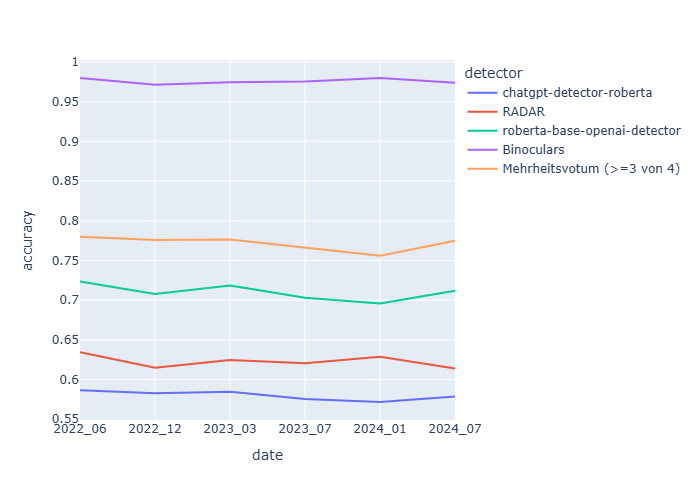
\includegraphics[width=\linewidth]{figures/plots/hauptexperiment/zeitverlauf/hauptexperiment_zeitverlauf_sample3000_accuracy.png}
      \caption{Accuracy im Zeitverlauf}
      \label{fig:1}
    \end{subfigure}\hfil % <-- added
    \begin{subfigure}{\textwidth}
      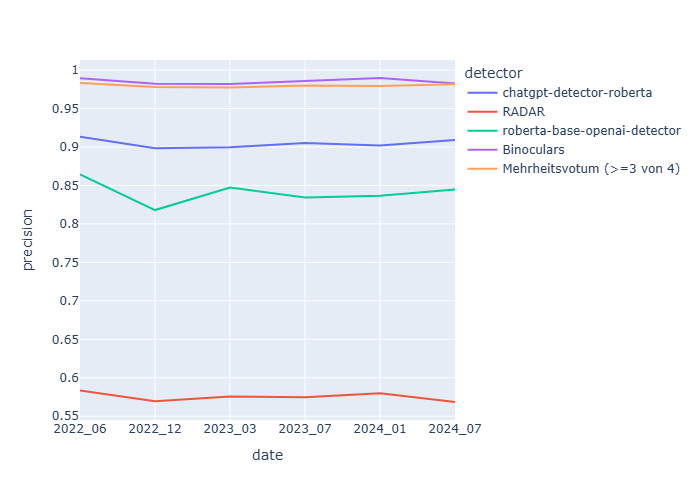
\includegraphics[width=\linewidth]{figures/plots/hauptexperiment/zeitverlauf/hauptexperiment_zeitverlauf_sample3000_precision.png}
      \caption{Precision im Zeitverlauf}
      \label{fig:2}
    \end{subfigure}\hfil % <-- added
    \begin{subfigure}{\textwidth}
      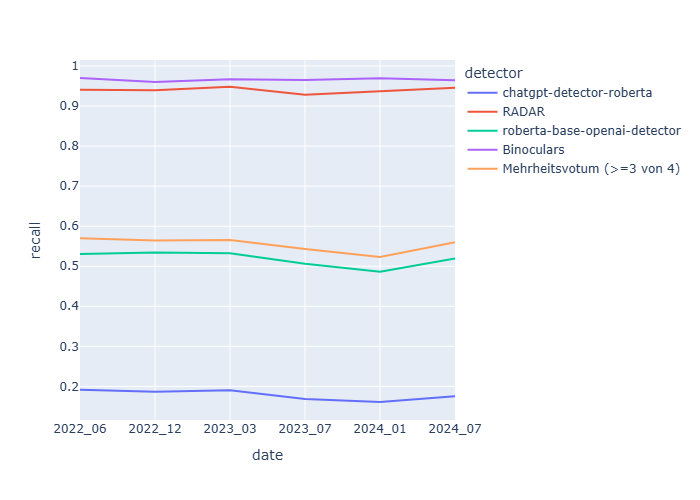
\includegraphics[width=\linewidth]{figures/plots/hauptexperiment/zeitverlauf/hauptexperiment_zeitverlauf_sample3000_recall.png}
      \caption{Recall im Zeitverlauf}
      \label{fig:3}
    \end{subfigure}
  \end{minipage}\hfil
  \begin{minipage}[t]{.5\textwidth}
    \begin{subfigure}{\textwidth}
      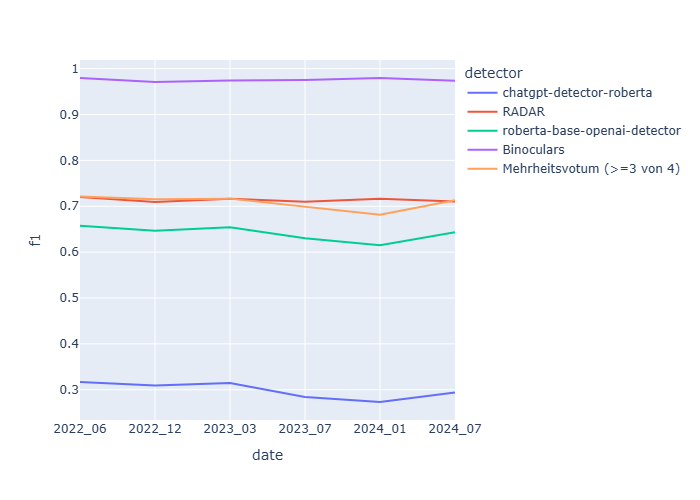
\includegraphics[width=\linewidth]{figures/plots/hauptexperiment/zeitverlauf/hauptexperiment_zeitverlauf_sample3000_f1.png}
      \caption{F1-Score im Zeitverlauf}
      \label{fig:4}
    \end{subfigure}\hfil % <-- added
    \begin{subfigure}{\textwidth}
      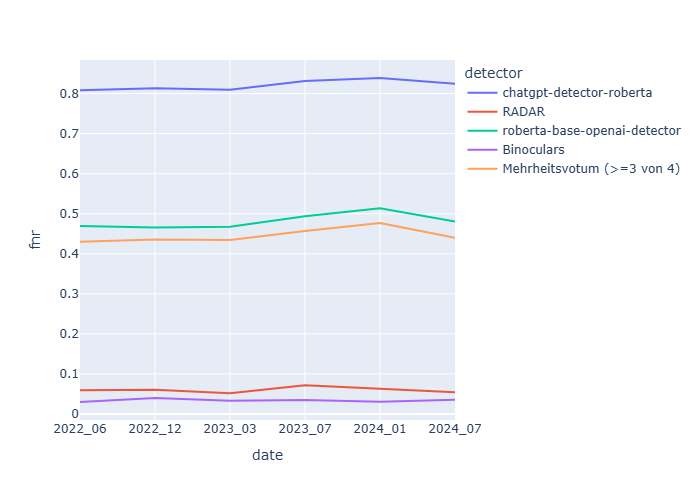
\includegraphics[width=\linewidth]{figures/plots/hauptexperiment/zeitverlauf/hauptexperiment_zeitverlauf_sample3000_fnr.png}
      \caption{FNR im Zeitverlauf}
      \label{fig:5}
    \end{subfigure}\hfil % <-- added
    \begin{subfigure}{\textwidth}
      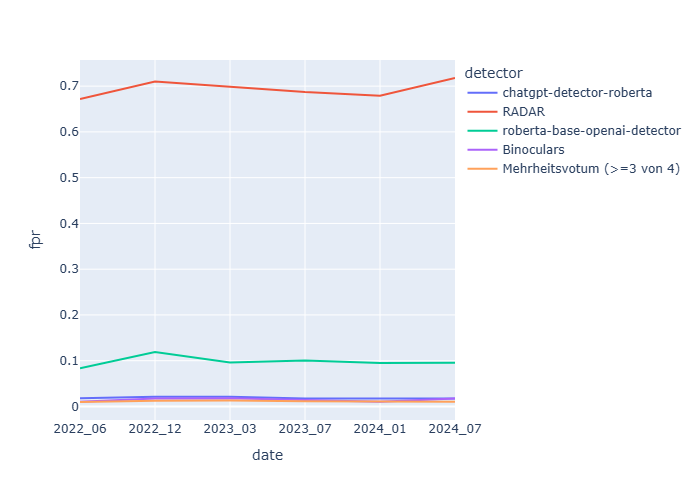
\includegraphics[width=\linewidth]{figures/plots/hauptexperiment/zeitverlauf/hauptexperiment_zeitverlauf_sample3000_fpr.png}
      \caption{FPR im Zeitverlauf}
      \label{fig:6}
    \end{subfigure}
  \end{minipage}
  \caption{Verwendete Metriken im Zeitverlauf für alle Detektoren}
  \label{fig:images}
\end{figure}
Alle Detektoren und auch das Ensemble mit Mehrheitsentscheid zeigen einen Anstieg der False Positive Rate beim Vergleich zwischen Juni 2022 und Dezember 2022 von bis zu 3,8 Prozentpunkten. Insgesamt lässt sich eine Tendenz von mehr False Positives zwischen dem frühesten und dem spätesten untersuchten Zeitpunkt beobachten. \textcolor{red}{(Interpration (muss später zu Diskussion): Dies könnte ein Hinweis darauf sein, dass tatsächlich mehr KI-generierte Posts unter den echten Posts sind.)} \\
Die Trefferquote, also der Recall, verhält sich für alle Detektoren und auch das Ensemble über die Zeit hinweg relativ stabil. Lediglich beim ChatGPT Detector RoBERTa, dem RoBERTa OpenAI Detector und dem Ensemble zeigt sich, dass im Januar 2024 im Vergleich zum Juni 2022 etwas weniger KI-Texte auch als solche erkannt werden (ChatGPT Detector RoBERTa: 19 \% im Juni 2022 vs. 16 \% im Januar 2024; RoBERTa OpenAI Detector: 53 \% im Juni 2022 vs. 49 \% im Januar 2024; Ensemble: 57 \% im Juni 2022 vs. 52 \% im Januar 2024). Im darauffolgenden Zeitpunkt, dem Juli 2024, steigen die Werte aber für beide Detektoren und das Ensemble wieder auf ein ähnliches Niveau im Vergleich zum Juni 2022. \\
Vergleicht man die Länge der realen Texte und der generierten Texte fällt auf, dass zu allen Zeitpunkten die generierten Texte im Mittel deutlich länger sind (siehe Abbildung~\ref{fig:textlength_zeitverlauf}).


\begin{figure}[H]
  \centering
  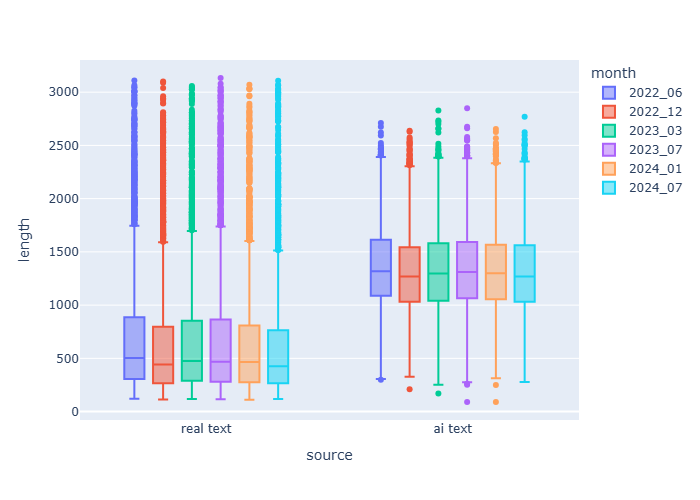
\includegraphics[width=0.6\textwidth]{figures/plots/hauptexperiment/zeitverlauf/hauptexperiment_zeitverlauf_sample3000_textlength.png}
  \caption[Textlänge im Zeitverlauf]{Vergleich der Textlänge im Zeitverlauf in der Stichprobe}
  \label{fig:textlength_zeitverlauf}
\end{figure}

Über die Zeiträume hinweg zeigt sich, dass die KI-generierten Texte vor der Trunkierung auf 1500 Zeichen im Mittel doppelt so lang sind wie die realen Posts (siehe Tabelle~\ref{table:vergleich_textlänge}). Wie oben beschrieben wurde (siehe Kapitel~\ref{subsec:Hauptexperiment}), soll neben dem Zeitverlauf auch der Einfluss der Textlänge auf die Detektionsleistung untersucht werden. Die Ergebnisse aus der Forschung legen nahe, dass ein positiver Zusammenhang zwischen Textlänge und Detektionsleistung besteht \autocite{chakraborty2023possibilitiesaigeneratedtextdetection,Rashidi_Fennell_Albahra_Hu_Gorbett_2023}. Um diesen Befund auf den mir vorliegenden Daten zu überprüfen, wird eine Stichprobe von jeweils 3.000 realen und künstlich generierten Posts mit verschiedenen Klassen von Textlängen gebildet.

\textcolor{red}{We further remark that it would be quite difficult to make LLMs exactly equal to human distributions due to the vast diversity within the human population, which may require a large number of samples from an information-theoretic perspective and provide a lower bound on the closeness distance to human distributions. \autocite{chakraborty2023possibilitiesaigeneratedtextdetection}}


\begin{table}[htbp]
  \centering
  \caption{Vergleich der Textlänge zwischen den beiden Klassen}
  \label{table:vergleich_textlänge}
  \begin{tabularx}{1.0\textwidth}{>{\raggedright\arraybackslash}X>{\raggedright\arraybackslash}X>{\raggedright\arraybackslash}X}
    \toprule
    \textbf{}          & \textbf{real text} & \textbf{ai text} \\
    \midrule
    Mittelwert         & 660,72             & 1332,38          \\
    Standardabweichung & 555,82             & 396,36           \\
    Minimum            & 112                & 90               \\
    Median             & 462                & 1295             \\
    Maximum            & 3133               & 2848             \\
    \bottomrule
  \end{tabularx}
\end{table}

In Abbildung~\ref{fig:textlaenge} lässt sich erkennen, dass prinzipiell ein positiver Zusammenhang zwischen der Textlänge und der Erkennungsleistung besteht, der aber zwischen den Detektoren und den beobachteten Metriken variiert. Eine Ausnahme von  diesem grundsätzlichen positiven Zusammenhang bildet RADAR im Hinblick auf False Negative Rate und Recall. Die False Negative Rate des Detektors steigt von 0,6 \% bei einer Textlänge von 0 bis 150 Zeichen auf rund 10,7 \% bei einer Textlänge von 750 bis 900 Zeichen. Der Wert für den Recall von RADAR sinkt im Vergleich zwischen diesen beiden Klassen an Textlängen von 99,4 \% um 10 Prozentpunkte auf 89,3 \%. RADAR weist für diese beiden Metriken dennoch über die Textlängen hinweg den höchsten (Recall) bzw. niedrigsten (FNR) Wert auf. Hinsichtlich der Accuracy fällt auf, dass die Leistung von Binoculars auf eher kürzeren Texten ähnlich zu den anderen Detektoren ist. Ab einer Länge von 150 bis 300 Zeichen steigt die Genauigkeit allerdings deutlich an und bewegt sich fortan auf einem höheren Niveau als die anderen Detektoren und der Mehrheitsentscheid. Interessant ist hierbei auch, dass für Texte zwischen 0 und 150 Zeichen der RoBERTa Base OpenAI Detector den höchsten Wert unter allen Detektoren und dem Ensemble hat. Danach sinkt dessen Leistung aber ab, wenn die Klasse mit einer Textlänge von 150 bis 300 Zeichen betrachtet wird. Werden die Texte daraufhin wieder länger, also ab 300 Zeichen, steigt die Genauigkeit des Detektors wieder an. Für den Recall, den F1-Score und die False Negative Rate zeigt sich für den RoBERTa Base OpenAI Detector ein jeweils ähnliches Bild. Hier sinken Recall und F1-Score zunächst bis zur Klasse der Texte mit Zeichenlängen zwischen 300 und 450 Zeichen und steigen anschließend mit zunehmender Textlänge. Analog dazu zeigt die FNR einen entgegengesetzten Verlauf. \\
Mit der Ausnahme der Klassen von 150 bis 300 Zeichen und 300 bis 450 Zeichen zeigt der ChatGPT Detector RoBERTa die niedrigste Genauigkeit über die unterschiedlichen Textlängen hinweg. Die Entwicklung der Precision des RoBERTa Base OpenAI Detectors zeigt eine Ähnlichkeit zum Verlauf der Accuracy ebenjenes Detektors. Auch hier gibt es einen „Knick“ in der Klasse von 150 bis 300 Zeichen und danach einen ansteigenden Verlauf. Auffallend ist auch die Precision von RADAR, die bis zu einer Zeichenzahl zwischen 300 und 450 Zeichen einen relativ konstanten Wert aufweist und danach bis auf einen Wert von 72,6 \% steigt.
Betrachtet man den Recall und die False Positive Rate, zeigt sich für RADAR ein auffälliges Verhältnis. Über alle Textlängenklassen hinweg weist dieser Detektor den höchsten Recall auf. RADAR klassifiziert also die überwiegende Mehrheit der KI-Texte korrekt. Gleichzeitig zeigt der Detektor jedoch die höchste False Positive Rate unter allen Detektoren und dem Mehrheitsentscheid. In den Klassen mit einer Textlänge zwischen 0 und 150 Zeichen bzw. 150 und 300 Zeichen erkennt RADAR fast alle menschlichen Texte fälschlich als KI-generiert. Zwar sinkt die FPR von 99,97 \% mit steigender Textlänge auf ein Niveau von 33,67 \% bei Texten mit einer Länge zwischen 750 und 900 Zeichen, liegt aber dennoch erheblich über den Werten der übrigen Detektoren und dem Ensemble. Die hohen Recall-Werte von RADAR gehen also mit einer hohen False Positive Rate einher, da der Detektor menschliche und auch KI-Texte als künstlich generiert identifiziert. Dieser Umstand spricht für die Annahme, dass RADAR besonders bei kurzen Texten stark dazu tendiert den Inhalt als KI-generiert zu klassifizieren. Damit kann auch die vergleichsweise niedrige Accuracy von RADAR vor allem bei kurzen Texten erklärt werden.
Der stärkste Effekt der Textlänge ist bei Binoculars neben der Accuracy auch beim F1-Score zu sehen, wo der Wert von 7,7 \% auf 89,1 \% steigt, während bei den anderen Detektoren der Zusammenhang auch, aber in mehr oder weniger deutlich geringerem Ausmaß erkennbar ist. Binoculars zeigt bei kürzeren Texten zunächst einen vergleichsweise niedrigen F1-Score, der sich aber ab der Textlängenklasse von 300 bis 450 Zeichen deutlich und kontinuierlich steigert. Vergleicht man die Precision und den Recall, zeigt sich, dass vor allem die Precision aller Detektoren mit zunehmender Textlänge insgesamt verbessert wird, während der Recall nicht bei allen Detektoren in gleichem Maß ansteigt. Binoculars zeigt eine Steigerung von ca. 40 Prozentpunkten von ca. 60 \% auf fast 100 \% im Hinblick auf die Precision und eine noch deutlichere Verbesserung der Erkennungsleistung in Bezug auf den Recall von knapp 4 \% auf rund 81 \%. Damit zeigt sich auch bei Binoculars für mehrere Metriken ein erkennbarer positiver Zusammenhang zwischen Textlänge und Detektionsleistung.
Das Ensemble liegt hinsichtlich der beobachteten Metriken über die Textklassen hinweg häufig zwischen den Einzeldetektoren und zeigt eine bessere Leistung als der jeweils schlechteste Einzeldetektor. Der Mehrheitsentscheid zeigt seine Stärken bei längeren Texten im Hinblick auf die Precision und die FPR. Die Accuracy und der F1-Score des Ensembles steigen ebenfalls mit zunehmender Textlänge. Für die längeren Textlängenklassen liegen die Werte für diese beiden Metriken für das Ensemble allerdings unter dem Niveau von Binoculars bzw. RADAR. \\
Zusammenfassend lässt sich sagen, dass für die evaluierten Detektoren überwiegend ein positiver Zusammenhang zwischen der Länge des Textes und der Detektionsleistung erkennbar ist. Die Stärke dieses Zusammenhangs schwankt allerdings deutlich je nach Detektor und beobachteter Metrik. Bei Binoculars ist der Zusammenhang am prägnantesten, während RADAR ein abweichendes Muster zeigt und bereits bei kurzen Texten einen sehr hohen Recall aufweist. Mit dem hohen Recall von RADAR geht jedoch eine hohe FPR des Detektors über alle Textlängenklassen hinweg einher. Das Ensemble zeigt zwar auch einen positiven Effekt der Textlänge auf die Erkennungsleistung, kann aber die jeweils stärksten Einzeldetektoren nicht übertreffen.
\begin{figure}[htb]
  \centering % <-- added
  \begin{minipage}[t]{.5\textwidth}
    \begin{subfigure}{\textwidth}
      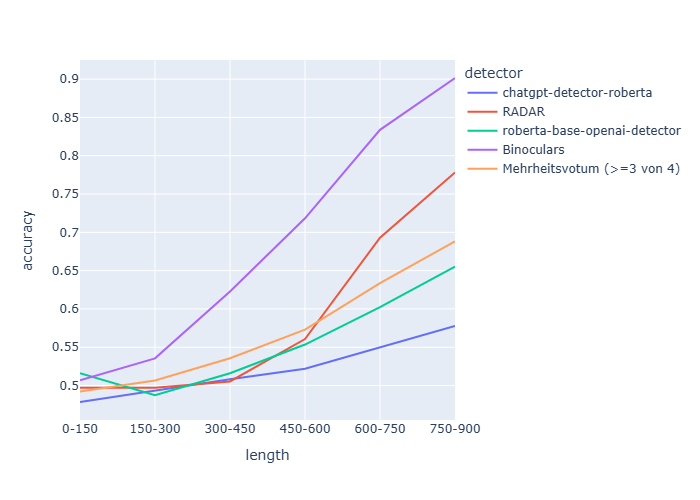
\includegraphics[width=\linewidth]{figures/plots/hauptexperiment/textlänge/hauptexperiment_textlänge_sample3000_accuracy.png}
      \caption{Accuracy nach Zeichenzahl}
      \label{fig:1}
    \end{subfigure}\hfil % <-- added
    \begin{subfigure}{\textwidth}
      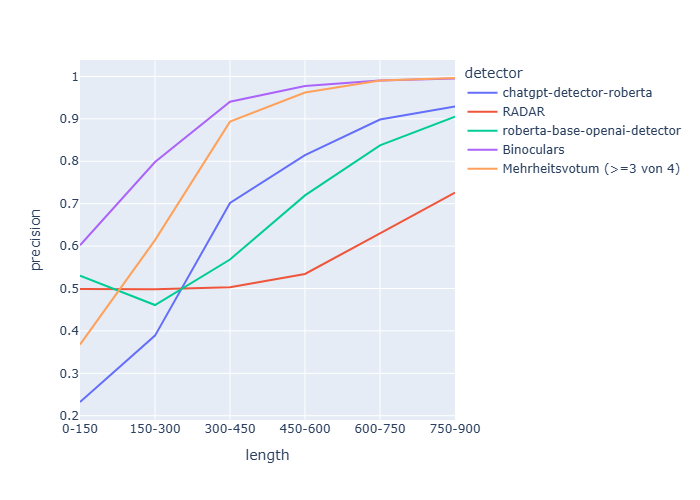
\includegraphics[width=\linewidth]{figures/plots/hauptexperiment/textlänge/hauptexperiment_textlänge_sample3000_precision.png}
      \caption{Precision nach Zeichenzahl}
      \label{fig:2}
    \end{subfigure}\hfil % <-- added
    \begin{subfigure}{\textwidth}
      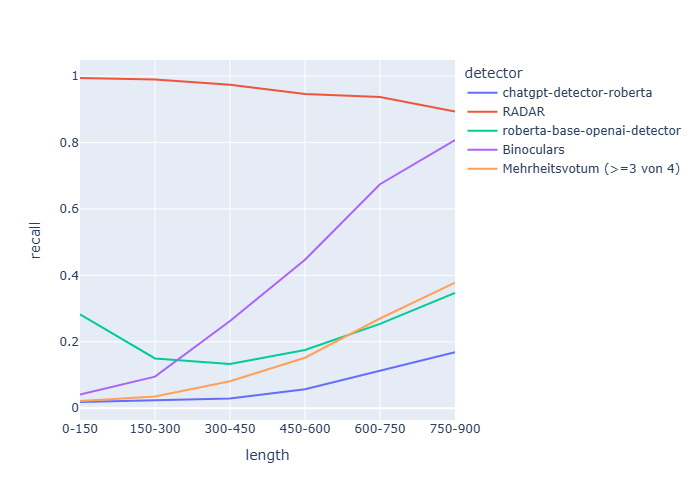
\includegraphics[width=\linewidth]{figures/plots/hauptexperiment/textlänge/hauptexperiment_textlänge_sample3000_recall.png}
      \caption{Recall nach Zeichenzahl}
      \label{fig:3}
    \end{subfigure}
  \end{minipage}\hfil
  \begin{minipage}[t]{.5\textwidth}
    \begin{subfigure}{\textwidth}
      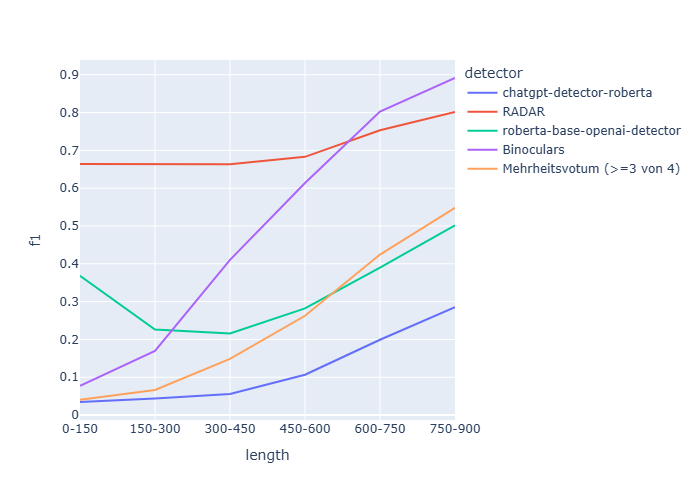
\includegraphics[width=\linewidth]{figures/plots/hauptexperiment/textlänge/hauptexperiment_textlänge_sample3000_f1.png}
      \caption{F1-Score nach Zeichenzahl}
      \label{fig:4}
    \end{subfigure}\hfil % <-- added
    \begin{subfigure}{\textwidth}
      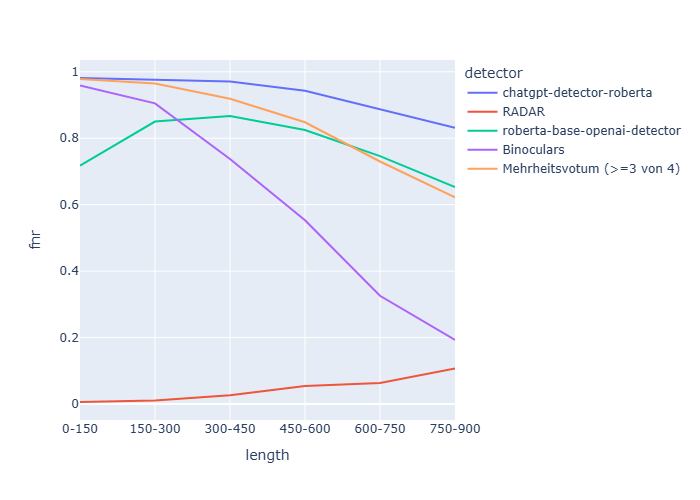
\includegraphics[width=\linewidth]{figures/plots/hauptexperiment/textlänge/hauptexperiment_textlänge_sample3000_fnr.png}
      \caption{FNR nach Zeichenzahl}
      \label{fig:5}
    \end{subfigure}\hfil % <-- added
    \begin{subfigure}{\textwidth}
      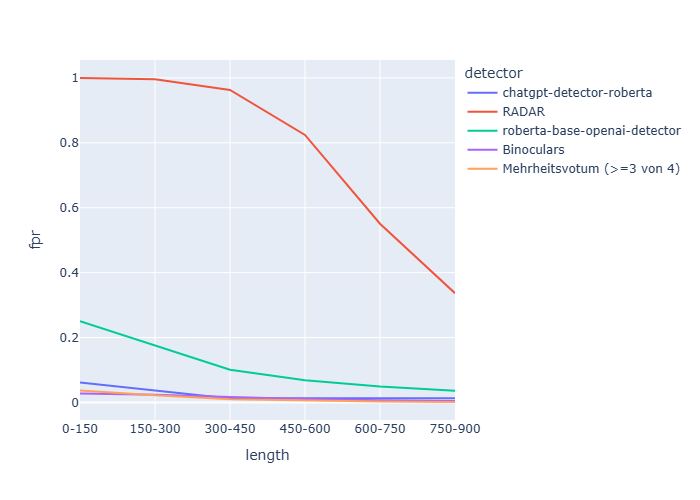
\includegraphics[width=\linewidth]{figures/plots/hauptexperiment/textlänge/hauptexperiment_textlänge_sample3000_fpr.png}
      \caption{FPR nach Zeichenzahl}
      \label{fig:6}
    \end{subfigure}
  \end{minipage}
  \caption{Verwendete Metriken nach Zeichenzahl für alle Detektoren}
  \label{fig:textlaenge}
\end{figure}


\chapter{Diskussion}
\label{chap:discussion}
Der folgende Abschnitt soll die Ergebnisse rekapitulieren, diskutieren und ihre Limitationen aufzeigen. \\
Im ersten Vorexperiment sollten die Detektoren auf einer Stichprobe von 1.000 Posts getestet werden. Hier zeigt sich, dass die Leistung der Detektoren auf der Stichprobe stark variiert. Am besten schneidet hierbei jedoch Binoculars ab, das über alle beobachteten Metriken die höchsten Werte erreicht und menschliche als auch KI-generierte Texte mit einer hohen Zuverlässigkeit klassifiziert. RADAR und der ChatGPT Detector RoBERTa zeigen entgegengesetzte Muster. Ersterer weist einen hohen Recall auf und erkennt somit viele KI-Texte korrekt. Gleichzeitig werden viele menschliche Texte fälschlich als KI-generiert klassifiziert. Der ChatGPT Detector RoBERTa erkennt die überwiegende Mehrheit der menschlichen Texte als solche. KI-Texte werden von diesem Detektor aber häufig nicht korrekt erkannt und als menschlich klassifiziert. Diese Ergebnisse zeigen, dass die Analyse einer einzelnen Evaluationsmetrik zu kurz greift, um die gesamte Erkennungsleistung zu beurteilen. Auffallend ist, dass der RoBERTa Base OpenAI Detector trotz seiner vergleichsweise veralteten und eingeschränkten Trainingsdaten hinsichtlich der betrachteten Metriken unter den experimentellen Bedingungen eine bessere Erkennungsleistung zeigt als der jeweils schlechteste Einzeldetektor. In Bezug auf die Zahl der False Negatives zeigen RADAR und Binoculars die niedrigsten Werte. Binoculars ist dabei allerdings besser in der Lage gleichzeitig auch die False Positive Rate niedrig zu halten. Somit ist Binoculars unter den im Vorexperiment untersuchten Bedingungen der zuverlässigste Detektor. Da hier allerdings nur ein Ausschnitt der Daten verwendet wurde und die Generierung ausschließlich mit LLaMA-3.1-8B-Instruct erfolgt ist, können die Ergebnisse nicht ohne Weiteres auf andere Texte und generierende Sprachmodelle übertragen werden.
Das Ensemble mit Mehrheitsentscheidung ist für die Metriken Accuracy, Precision und F1-Score leistungsstärker als alle Einzeldetektoren mit der Ausnahme von Binoculars.
Der deutlich geringere Recall des Ensembles im Vergleich zu Binoculars weist darauf hin, dass bei einem beträchtlichen Teil der KI-generierten Texte nicht mindestens drei der vier Detektoren gleichzeitig für eine KI-Klassifikation stimmen. Es könnte sein, dass die hohe Zahl der False Negatives des ChatGPT Detector RoBERTa hierzu beiträgt. Wenn das Ensemble einen Text als KI-generiert erkennt, stimmt diese Entscheidung im Großteil der Fälle. Allerdings werden über 40 \% der KI-generierten Texte nicht als solche erkannt. Auf Basis dieser Stichprobe und den untersuchten Bedingungen kann das hier zugrundeliegende Ensemble mit einer \(\frac{3}{4}\)-Mehrheitsentscheidung nicht die Leistung des starken Einzeldetektors Binoculars übertreffen. Die hier verwendete Kombination mehrerer Detektoren zu einem Ensemble mit \(\frac{3}{4}\)-Mehrheitsentscheidung kann also die Schwächen der Einzeldetektoren nicht ausreichend ausgleichen, auch nicht bei der Verwendung von Binoculars als starkem Detektor. Im hier durchgeführten Vorexperiment gehen die Detektoren alle gleichermaßen in die Mehrheitsentscheidung ein. Alternativ könnte man die performanteren Detektoren höher gewichten und so deren Einfluss auf das Mehrheitsvotum stärken.
Unter diesen Bedingungen lässt sich die Hypothese \hyperlink{hp:2}{H\textsubscript{2}} vorläufig nicht bestätigen. Allerdings müssen diese Ergebnisse vor dem Hintergrund der Beschränkung auf Posts aus nur einem einzelnen Monat und der ausschließlichen Verwendung von LLaMA-3.1-8B-Instruct zur Textgenerierung gesehen werden. \\
Im zweiten Vorexperiment sollten KI-Verdächtigungen in den Kommentaren quantifiziert werden. Dies sollte anhand einer Schlagwortsuche mit Hilfe von Regular Expressions erfolgen. Im Ergebnis zeigte sich anhand der verwendeten Regex-Muster im gesamten Untersuchungszeitraum zwischen Januar 2022 und Dezember 2024, dass nur ein sehr kleiner Teil der Kommentare als KI-Verdächtigung identifiziert wird. Prinzipiell lässt sich zwar ein leichter Anstieg über die Zeit hinweg beobachten, allerdings weist der Verlauf starke Schwankungen auf. Dieser leichte Anstieg könnte in Zusammenhang mit der zunehmenden Verbreitung von LLMs stehen. Des Weiteren können sich die Formulierungen und Begriffe in diesem Kontext verändert haben. Beispielhaft dafür ist der Begriff „ai slop“, dessen Verwendung im Laufe der Jahre in englischsprachigen sozialen Medien deutlich zugenommen hat und ältere ähnlich abwertende Begriffe in diesem Kontext abgelöst hat \autocite{miklian2026s}. In diesem Sinne könnte ein Teil des Anstiegs damit erklärt werden, dass Begriffe wie „ChatGPT“ und „ai-generated“ erst mit der zunehmenden Prominenz von ChatGPT und generativen KI-Modellen im Allgemeinen vermehrt in den Sprachgebrauch aufgenommen wurden. Generell lässt sich in bestimmten Subreddits eine ablehnende Haltung gegenüber KI-generierten Inhalten erkennen, was dazu führen könnte, dass häufiger KI-Verdächtigungen ausgesprochen werden. Dies könnte insbesondere der Fall bei Subreddits sein, die auf menschlich produzierte Inhalte Wert legen und diese auch in ihren Regeln festlegen, wie „r/changemyview“ oder „r/WritingPrompts“ \autocite{lloyd2025there}.
Insgesamt sind die absoluten Häufigkeiten von KI-Verdächtigungen sehr gering und erschweren damit die Interpretation der zeitlichen Entwicklung. Die vergleichsweise großen Unterschiede in den relativen Werten können bereits durch geringe Schwankungen in den absoluten Zahlen der identifizierten KI-Verdächtigungen ausgelöst werden. In Anbetracht dessen muss auch die Interpretation des leichten Anstiegs mit Bedacht erfolgen. Ein Grund für die geringe absolute Anzahl an KI-Verdächtigungen im vorliegenden Datensatz, könnte die Auswahl der Regex-Muster sein. Diese berücksichtigen ausschließlich deutsch- und englischsprachige Kommentare und decken nicht alle in den Reddit-Kommentaren vorhandenen Sprachen ab. Es könnte also sein, dass die Zahl der KI-Verdächtigungen durchaus höher liegt, wenn die Regex-Muster auch um andere Sprachen ergänzt werden. Außerdem könnte es sein, dass die konkret untersuchten Formulierungen deutlich von den gängigen auf Reddit verwendeten Phrasen abweichen. Kommentare können zwar die untersuchten Phrasen enthalten, aber dennoch keine KI-Verdächtigung als solche gegenüber einem Post oder Kommentar äußern. Dies kann der Fall sein, wenn der Verfasser des Kommentars eine Phrase nutzt, die aber im Kontext einer allgemeinen Diskussion zum Thema KI verwendet wird, ohne einen konkreten Verdacht zu äußern. Zudem können besonders kurze Muster fälschlicherweise Treffer in anderen Sprachen als Englisch oder Deutsch erzeugen, wenn diese dort eine andere Bedeutung haben (Beispiel: „ai post“ auf Italienisch). Die verwendeten Regular Expressions können somit sowohl zu False Positives als auch False Negatives führen. Zusammenfassend kann gesagt werden, dass die hier festgestellte Anzahl an Treffern auf Grundlage von Regular Expressions nicht zwangsläufig der Anzahl an tatsächlich geäußerten Verdächtigungen entspricht. Das Vorexperiment stellt lediglich einen Versuch der Abschätzung dar und erfasst zunächst nur sprachliche Hinweise auf KI-Verdächtigungen. Auf Basis der Ergebnisse des zweiten Vorexperiments stellt sich auch die Frage, wie sich KI-Verdächtigungen in natürlicher Sprache in Form von Kommentaren identifizieren lassen. Eine einfache Schlagwortsuche, wie sie hier verwendet worden ist, könnte nicht ausreichend sein, um eine zuverlässige Erkennung zu ermöglichen. Es wäre denkbar, dass eine Zero-Shot-Klassifikation über Natural Language Inference (NLI)-Ansätze, die Verwendung von LLMs oder ein Fine-Tuning bestehender Klassifikatoren eine sinnvolle Ergänzung darstellen könnten. Diese sind eventuell besser in der Lage bestimmte potenzielle Phrasen der Verdächtigung im Kontext zu sehen. Zu erwähnen ist auch, dass sich diese Ergebnisse nicht auf die Grundgesamtheit aller auf Reddit veröffentlichten Kommentare übertragen lassen. Es werden aus bestimmten Monaten nur Stichproben betrachtet und manche Monate enthalten ohnehin nur 100.000 Kommentare. \\
Das erste Vorexperiment diente als Maßgabe für das weitere Vorgehen in dieser Arbeit. Da vor allem Binoculars auf der untersuchten Stichprobe gute Ergebnisse erzielt hat und auch die anderen Modelle in gewissen Bereichen ihre Stärken haben, sollen alle Detektoren im Hauptexperiment auf einer größeren Stichprobe evaluiert werden. Hierzu wurden zunächst verschiedene Zeitpunkte betrachtet. Diese Zeitpunkte sollen sich an Meilensteinen in der Entwicklung und der Verbreitung von LLMs orientieren. Für alle Zeitpunkte wird zur Generierung immer LLaMA-3.1-8B-Instruct verwendet. Es wird also nicht unmittelbar die technische Weiterentwicklung der LLMs über die Zeit hinweg abgebildet. Vielmehr wird untersucht, ob ein Zusammenhang zwischen dem Veröffentlichungszeitraum der zugrunde liegenden Posts bzw. deren möglicher Veränderung über die Zeit und der Leistung der Detektoren besteht. Dabei diente der Juni 2022 als Referenzzeitpunkt vor der Veröffentlichung von ChatGPT. Es kann davon ausgegangen werden, dass zu diesem Zeitpunkt die Verbreitung von LLMs sehr beschränkt war. Die darauffolgenden Zeitpunkte wurden so gewählt, dass sie die großen Weiterentwicklungsschritte von LLMs abbilden. Aus diesem Grund wurden der Dezember 2022 (Veröffentlichung ChatGPT), der März 2023 (Veröffentlichung GPT-4), der Juli 2023 (Veröffentlichung LLaMA 2), der Januar 2024 und der Juli 2024 (Veröffentlichung LLaMA-3.1) als weitere Zeitpunkte untersucht. Aus jedem dieser Monate wurde eine Stichprobe von 3.000 Posts gezogen, auf deren Basis dann ebenso wie in Vorexperiment 1 mithilfe von LLaMA-3.1-8B-Instruct künstliche Posts generiert wurden. \\
Zunächst sollte vermutet werden, dass so gut wie alle menschlichen Posts in der Stichprobe aus dem Juni 2022 von den Detektoren auch als solche klassifiziert werden. Allerdings haben bereits zu diesem Zeitpunkt alle Detektoren in mehr oder weniger großem Ausmaß menschlichen Text als KI erkannt. Besonders auffällig ist in diesem Kontext die False Positive Rate von RADAR. Dieser Detektor erkennt in der Stichprobe aus dem Juni 2022 67 \% der von Menschen verfassten Posts fälschlicherweise als KI-generiert. Auch über alle anderen untersuchten Zeiträume weist RADAR die mit Abstand höchste FPR auf. Hier wird dieselbe Problematik verdeutlicht, die bereits im ersten Vorexperiment beobachtet werden konnte. RADAR hat nach Binoculars den höchsten Recall und klassifiziert gleichzeitig auch einen erheblichen Teil der menschlichen Texte fälschlicherweise als KI-generiert. Dies legt nahe, dass RADAR unter den hier verwendeten experimentellen Bedingungen bestimmte Merkmale von menschlichen Reddit-Posts als Indikatoren für KI-generiertem Text interpretiert. In weniger ausgeprägter Form könnte dies auch bei den anderen Detektoren der Fall sein. Die FPR des ChatGPT Detector RoBERTa und von Binoculars bewegen sich über die betrachteten Zeitpunkte hinweg auf einem ähnlich niedrigen Niveau. Beide Detektoren erkennen also menschlichen Text am zuverlässigsten auch als solchen. Gleichzeitig gibt es aber einen deutlichen Unterschied im Recall. Der ChatGPT Detector RoBERTa erkennt nur rund 20 \% der KI-generierten Texte auch als solche, während Binoculars einen Recall von deutlich über 90 \% erreicht. Die hohe Diskrepanz zwischen der FPR und dem Recall des ChatGPT Detector RoBERTa deutet darauf hin, dass der Detektor in seiner Klassifikation eher zurückhaltend ist. Nur wenige menschliche Texte werden fälschlich als KI-generiert erkannt und gleichzeitig werden nur wenige der tatsächlich KI-generierten Texte als solche klassifiziert. Auch hier zeigt sich, dass eine Metrik alleine nicht ausreicht, um die Leistung eines Detektors hinreichend zu beurteilen.\\
Über die untersuchten Zeiträume hinweg lässt sich nur eine sehr schwache Veränderung in der Erkennungsleistung beobachten. Die Metriken verhalten sich für alle evaluierten Detektoren überwiegend stabil. Außerdem sind in der untersuchten Stichprobe keine wesentlichen Unterschiede in der Rangfolge der Detektoren erkennbar. Es zeigt sich unter den gegebenen experimentellen Bedingungen und der gewählten Stichprobe keine auffällige Leistungssteigerung oder -abfall der Detektoren über die Zeit hinweg. Zwar lassen sich für einzelne Detektoren kleine Unterschiede hinsichtlich der FPR zwischen den Stichproben aus dem Juni und dem Dezember 2022 erkennen, aber daraus kann nicht ohne Weiteres ein Effekt der Veröffentlichung von ChatGPT geschlossen werden. Dazu müssten zusätzliche Zeitpunkte vor und nach Dezember 2022 betrachtet werden. Es kann zudem nicht ausgeschlossen werden, dass diese Fluktuationen auf unterschiedliche Subreddits, Textlängen und allgemein Stichprobenzusammensetzungen zurückzuführen sind. Hierzu müsste eine Kontrolle dieser Einflussfaktoren erfolgen. Auch hinsichtlich der Unterschiede im Recall der Detektoren zwischen den Stichproben aus Januar und Juli 2024 lässt sich nicht schlussfolgern, dass die Leistung der Detektoren über die Zeit hinweg abnimmt. In der Stichprobe aus Juli 2024 steigen die Werte wieder an und der vorhergehende Rückgang kann ebenfalls durch andere Eigenschaften des untersuchten Textes wie Textlänge und Subreddit beeinflusst worden sein.
Insgesamt zeigt sich Binoculars auch auf der größeren Stichprobe über alle beobachteten Monate und verwendeten Metriken hinweg als der zuverlässigste Detektor. Die Unterschiede zwischen den Detektoren scheinen stärker zu sein als die Differenzen zwischen den hier untersuchten Zeitpunkten. Es lässt sich also unter den gegebenen experimentellen Bedingungen kein eindeutiger Zusammenhang zwischen dem Veröffentlichungszeitraum der Reddit-Posts und der Erkennungsleistung der Detektoren feststellen. Zu berücksichtigen ist dabei, wie oben geschildert, dass für alle beobachteten Zeitpunkte dasselbe Modell, LLaMA-3.1-8B-Instruct, zur Generierung verwendet wurde. Die Ergebnisse zeigen daher nicht, wie sich die Leistung der Detektoren im Vergleich zu den jeweils tatsächlich verfügbaren LLMs entwickelt hat. Vielmehr zeigen sie, inwiefern die Erkennungsleistung variiert, wenn die menschlichen Reddit-Posts aus unterschiedlichen Veröffentlichungszeiträumen stammen. \\
Im zweiten Teil des Hauptexperiments sollte der Einfluss der Textlänge auf die Detektionsleistung untersucht werden. Dazu wurden zunächst verschiedene Klassen an Textlängen gebildet (0-150, 150-300, 300-450, 450-600, 600-750, 750-900 Zeichen). Anschließend wurde für jede Textlängenklasse eine Stichprobe von jeweils 3.000 realen und KI-generierten Posts gebildet. Die Posts stammen aus denselben Monaten, die bereits im ersten Teil des Hauptexperiments verwendet wurden. Grundsätzlich ist ein positiver Zusammenhang zwischen der Textlänge und der Erkennungsleistung erkennbar. Allerdings gibt es Unterschiede zwischen den beobachteten Detektoren und den untersuchten Metriken. Insgesamt zeigt sich, dass mit längeren Texten offenbar auch mehr Informationen geliefert werden, die von den verwendeten Detektoren sinnvoll zur Klassifikation genutzt werden können. Sind die Texte sehr kurz, haben die Detektoren nur wenige Merkmale zur Verfügung anhand derer sie menschlichen von KI-generiertem Text unterscheiden können. Je länger der Text wird, desto eher steigt die Zahl von potenziell relevanten Mustern in Vokabular, Syntax und statistischen Regelmäßigkeiten. Betrachtet man die Accuracy und F1-Score fällt auf, dass vor allem Binoculars mit einer zunehmenden Textlänge auch deutlich bessere Ergebnisse liefert. Dies könnte dadurch erklärt werden, dass dieser Detektor diese Muster in längerem Text besser erkennt und nutzen kann. Für kürzere Texte weist Binoculars allerdings eine ähnlich eingeschränkte Zuverlässigkeit auf wie die anderen untersuchten Detektoren. Binoculars zeigt interessanterweise auch eine sichtliche Steigerung der Werte für den Recall und die Precision. Somit werden bei längeren Texten erstens mehr KI-generierte Texte richtig klassifiziert und zweitens auch mehr KI-Texte insgesamt erkannt. Auch dies deutet darauf hin, dass die Zuverlässigkeit von Binoculars bei kurzen Reddit-Posts nur sehr limitiert ist und in diesen Fällen die Ergebnisse deshalb nur mit Vorsicht interpretiert werden sollten. Anders verhält sich RADAR hinsichtlich Recall und FPR. Ähnlich wie oben bei Betrachtung zu unterschiedlichen Zeitpunkten weist RADAR hier über alle betrachteten Textlängen hinweg den höchsten Recall auf. Dass RADAR bei kurzen Texten einen hohen Recall zeigt, hängt vermutlich nicht damit zusammen, dass der Detektor besonders gut in der Lage ist KI-generierten Text zu erkennen, sondern eher, dass RADAR generell häufig für das Label „KI-generiert“ stimmt. Dafür spricht auch die sehr hohe FPR bei kurzen Texten. Diese sinkt zwar mit zunehmender Textlänge sichtlich, verläuft aber auch bei längeren Posts deutlich oberhalb der FPR der anderen untersuchten Detektoren. Werden die Texte länger, scheint RADAR für sich genommen besser in der Lage zu sein zwischen menschlichen und KI-generierten Posts zu differenzieren. Der Kurvenverlauf für die Accuracy, die Precision und den F1-Score des RoBERTa Base OpenAI Detectors spricht für diesen Detektor dafür, dass der Zusammenhang zwischen der Textlänge und der Detektionsleistung nicht unbedingt monoton ist. Auch hier könnte nicht nur die Textlänge einen Einfluss haben, sondern daneben auch Komponenten wie Stichprobenzusammensetzung oder Subreddit-spezifische Eigenheiten eine Rolle spielen. Für das Ensemble gelten hinsichtlich der Korrelation zwischen Textlänge und Erkennungsleistung ähnliche Tendenzen. Mit längeren Texten geht zwar eine bessere Erkennungsleistung einher, aber diese überbietet nicht die stärksten Einzeldetektoren. Insgesamt profitieren zwar alle untersuchten Modelle von längeren Texten und damit mehr Informationen, aber die Schwächen einzelner Detektoren werden aufgrund der \(\frac{3}{4}\)-Mehrheitsentscheidung auch hier nicht hinreichend ausgeglichen. Außerdem lässt sich unter den hier betrachteten experimentellen Bedingungen kein Kausaleffekt der Textlänge auf die Erkennungsleistung attestieren. Dazu bedarf es der Kontrolle anderer möglicher Einflussfaktoren.

\chapter{Fazit}
\label{chap:conclusion}

Hervorheben, dass es sich um ein experimentelles Vorgehen handelt

Punkte für weitere Forschung
\begin{itemize}
    \item Andere generierende Modelle verwenden, vielleicht auch gekoppelt an die jeweiligen Zeiträume
    \item Regex-Muster um weitere Sprachen erweitern
    \item NLI (Natural Language Inference) oder Encode-Decoder-Modelle wie LLaMA oder GPT zur Klassifikation nutzen
\end{itemize}


\appendix
\pagestyle{plain}

\printbibliography[heading=bibintoc]
\chapter*{Ehrenwörtliche Erklärung}
\label{declaration}

Hiermit erkläre ich, dass ich die vorliegende Bachelorarbeit selbständig verfasst, noch nicht anderweitig für Prüfungszwecke vorgelegt, keine anderen als die angegebenen Quellen oder Hilfsmittel benützt sowie wörtliche und sinngemäße Zitate als solche gekennzeichnet habe.

\vspace{1.5cm}
\begin{tabular*}{\textwidth}{%
    @{\extracolsep{\fill}}
    w{l}{5.5cm}
    c
    w{l}{5.5cm}
    @{}
  }
  München, \today && \includegraphics[height=1.3cm]{figures/logos/Unterschrift.png} \\
  \cmidrule(r){1-1}\cmidrule(l){3-3}
  Ort, Datum && Unterschrift
\end{tabular*}

\addcontentsline{toc}{chapter}{Ehrenwörtliche Erklärung}
\begin{appendices}

  \chapter{Anhang}
  \label{appendix}

  \section{Zusätzliches Material}

  \begin{table}[htbp]
    \centering
    \caption{Stichprobengrößen der untersuchten Veröffentlichungszeitpunkte}
    \label{tab:sample_size_hauptexperiment_zeitverlauf}
    \begin{tabularx}{1.0\textwidth}{>{\raggedright\arraybackslash}X>{\raggedright\arraybackslash}X}
      \toprule
      \textbf{Veröffentlichungszeitpunkt} & \textbf{Stichprobengröße} \\
      \midrule
      Juni 2022                           & 2.965                     \\
      Dezember 2022                       & 2.978                     \\
      März 2023                           & 2.959                     \\
      Juli 2023                           & 2.946                     \\
      Januar 2024                         & 2.968                     \\
      Juli 2024                           & 2.962                     \\
      \bottomrule
    \end{tabularx}
  \end{table}

  \begin{table}[htbp]
    \centering
    \caption{Stichprobengrößen der untersuchten Veröffentlichungszeitpunkte}
    \label{tab:checkpoints_detectors}
    \begin{tabularx}{1.0\textwidth}{>{\raggedright\arraybackslash}X>{\raggedright\arraybackslash}X}
      \toprule
      \textbf{Veröffentlichungszeitpunkt} & \textbf{Stichprobengröße} \\
      \midrule
      RoBERTa Base OpenAI Detector        & 2.965                     \\
      ChatGPT Detector RoBERTa            & 2.978                     \\
      März 2023                           & 2.959                     \\
      Juli 2023                           & 2.946                     \\
      Januar 2024                         & 2.968                     \\
      Juli 2024                           & 2.962                     \\
      \bottomrule
    \end{tabularx}
  \end{table}

\end{appendices}


\end{document}
